\documentclass[10pt,a4paper]{article}
\usepackage[margin=2.0cm]{geometry}
\usepackage{microtype}
\usepackage{xurl}
\renewcommand{\UrlBreaks}{}
\def\ttbreaks{\allowbreak}
\usepackage{array}
\usepackage{ragged2e}
\setlength{\tabcolsep}{4pt}
\renewcommand{\arraystretch}{1.15}
\usepackage{booktabs}
\usepackage{array}
\usepackage{graphicx}
\usepackage{listings}
\usepackage{amsmath}
\usepackage{hyperref}
\usepackage[compact]{titlesec}
\hypersetup{colorlinks=true,linkcolor=blue,urlcolor=blue}
\lstset{basicstyle=\ttfamily\footnotesize,breaklines=true,breakatwhitespace=false,frame=single,columns=fullflexible,xleftmargin=0pt}

\title{Model Changes and Findings --- Limmattal Bike Highway\\[2pt]
\large Internal working report: exact variables changed, current results, and what the figures show}
\date{20 November 2026}

\begin{document}
\sloppy
\maketitle
\tableofcontents

\section{What this repo is}
Fork of the ETH IP-HS26 course repo. Upstream models the SBB MehrSpur rail project
(Z\"urich--Winterthur, Br\"uttenertunnel + stations). The fork swaps the case to a
Limmattal bike highway: Stage~1 = separated bike highway Z\"urich (Altstetten)--Schlieren,
Stage~2 = five additional underpasses. Notebooks 02--05 run the standard pipeline:
deterministic system model $\to$ uncertainty/surrogate $\to$ adaptive planning (200
scenarios $\times$ 6 plans, 40-year horizon) $\to$ cost-benefit appraisal at 2\%/yr.

All notebooks were re-executed end-to-end on 2026-11-20 after the changes below
(NB02 354\,s, NB03 32.9\,min including a full surrogate retrain, NB04 67\,s, NB05 77\,s;
zero error cells; UV-managed Python 3.11.17).

\section{Exact variables and values changed}

\subsection{Corridor and network (\texttt{code/parameters.py})}
\begin{center}\small\begin{tabular}{@{}>{\RaggedRight\arraybackslash}p{4.6cm}>{\RaggedRight\arraybackslash}p{3.4cm}>{\RaggedRight\arraybackslash}p{4.6cm}>{\RaggedRight\arraybackslash}p{3.0cm}@{}}
\toprule
Variable & upstream (MehrSpur) & current (bike case) & note \\
\midrule
CORRIDOR\_REGIONS / \_MUNICIPALITIES & 9 municipalities & emptied (zones mode) & \\
CORRIDOR\_DEFINITION\_MODE & \texttt{"municipalities"} & \texttt{"zones"} & \\
PROJECT\_ZONES & --- & 110 zone IDs (key \texttt{"Zurich\_S18\_Alignment"}) & \\
DETAILED\_NETWORK\_FILE & \texttt{mehrspur\_...pkl} & \texttt{bike\_highway\_...pkl} & OSM rebuilt \\
SECTION.active / crowding & True / True & False / False & no PT section in bike case \\
EXTERNAL\_FLOW.enabled / trips & True / 53{,}108 & False / 0 & \\
\bottomrule
\end{tabular}\end{center}

\subsection{Uncertainty ranges (\texttt{STRUCTURAL\_UNCERTAINTIES})}
\begin{center}\small\begin{tabular}{@{}>{\RaggedRight\arraybackslash}p{4.8cm}>{\RaggedRight\arraybackslash}p{3.2cm}>{\RaggedRight\arraybackslash}p{3.2cm}>{\RaggedRight\arraybackslash}p{4.4cm}@{}}
\toprule
Parameter & upstream min--max & current min--max & note \\
\midrule
PASSENGER\_DEMAND\_GROWTH (triangular, transient) & $-0.20$ -- $0.50$ & $\mathbf{-0.20 -- 0.50}$ & \textbf{reverted to upstream 2026-11-20} (was 0.078--0.251) \\
PT\_ASC\_SHIFT & $-0.10$ -- $0.30$ & $-0.10$ -- $0.30$ & unchanged \\
BIKE\_ASC\_SHIFT & commented out ($-0.50$--$1.00$) & \textbf{active}, $-0.50$--$1.00$ & enabled for bike case \\
EBIKE\_SHARE & $0.35$ -- $0.80$ & $0.23$ -- $0.72$ & narrowed \\
ROAD\_FREIGHT\_GROWTH & sigma-based & same structure & \\
\bottomrule
\end{tabular}\end{center}

\subsection{Valuation and appraisal parameters (\texttt{NOMINAL\_PARAMS})}
\begin{center}\small\begin{tabular}{@{}>{\RaggedRight\arraybackslash}p{4.4cm}>{\RaggedRight\arraybackslash}p{2.6cm}>{\RaggedRight\arraybackslash}p{4.2cm}>{\RaggedRight\arraybackslash}p{4.4cm}@{}}
\toprule
Parameter & upstream & current & source/comment \\
\midrule
PT\_SHARE\_TARGET & 0.35 & 0.47 & kept (stale comment); NB03 vulnerability rule \\
EBIKE\_SPEED\_MULTIPLIER & 1.5 & 1.54658 & kept (unexplained retune) \\
C\_NOISE\_CAR & 0.01490 & 0.0116 & kept \\
C\_ACCIDENT\_CAR & 0.08441 & 0.084441 & kept \\
C\_FLEX (option premium) & 50{,}000{,}000 CHF & 1{,}000{,}000 CHF & rescaled to project scale (code comment) \\
BENEFIT\_HEALTH\_BIKE\_PER\_KM & commented (1.0) & \textbf{1.306 CHF/pkm active} & Kanton Z\"urich (2017) \\
C\_TT\_BIKE\_LANE & --- & 24.5 CHF/h (34\% below 35.0) & new, bike case \\
C\_ACCIDENT\_BIKE / \_LANE & --- & 0.39 / 0.25 CHF/pkm & new, marked ``new'' \\
C\_TT\_BIKE (cycling VOT) & 35.0 & \textbf{18.7} & 2026-11-21: sensitivity test; see variant section \\
DISCOUNT\_RATE & 2\% & \textbf{4\%} & 2026-11-21 stress value: punishes early capex \\
OPEX\_RATE & 2\% & \textbf{4\%} & 2026-11-21: KPMG Swiss opex analysis, rounded up from 0.3x\% \\
\bottomrule
\end{tabular}\end{center}

\subsection{Infrastructure stages (\texttt{code/stages.py})}
Code block of the current Stage definitions (lines 175--235):
\begin{lstlisting}
PACKAGES = {
    "stations": {
        "name": "Stage 1 - Bike Highway Zurich-Schlieren",
        "bike_highways": [{
            "od_pairs": BIKE_HIGHWAY_OD_PAIRS,   # all corridor-zone OD pairs, built in get_stages()
            "both_directions": True,             # changed 2026-11-20 (was False)
            "min_distance_km": 0.0,
            "max_distance_km": 15.0,             # changed 2026-11-20 (was 1000.0)
            "effects": {"distance_reduction_pct": 5.0,
                        "speed_increase_pct": 100 * (16 / 13 - 1)}   # 13 -> 16 km/h
        }],
        "appraisal": {"capital_cost_chf": 28_422_872 + 2_681_000,  # 31.1M (upstream: 925M)
                      "lifetime_years": 80, "capital_share": 0.60},
    },
    "tunnel": {
        "name": "Stage 2 - Additional underpasses",
        "bike_highways": [{
            "od_pairs": BIKE_HIGHWAY_OD_PAIRS,
            "both_directions": True,             # changed 2026-11-20 (was False)
            "min_distance_km": 0.0,
            "max_distance_km": 15.0,             # changed 2026-11-20 (was 1000.0)
            "effects": {"speed_increase_pct": 100 * (18 / 16 - 1)}    # 16 -> 18 km/h
        }],
        "appraisal": {"capital_cost_chf": 2_688_120,  # (upstream tunnel: 2302.6M)
                      "lifetime_years": 80, "capital_share": 0.60},
    },
}
\end{lstlisting}
Zone selectors above the packages: \texttt{ALTSTETTEN\_ZONE\_IDS} (24 IDs),
\texttt{DIETIKON\_ZONE\_IDS} (27 IDs), \texttt{BIKE\_HIGHWAY\_AREA\_PAIR}; a helper
\texttt{\_all\_corridor\_od\_pairs()} builds all ordered pairs of the 110 corridor zones
and \texttt{\_assemble\_stages} injects them wherever an intervention has
\texttt{od\_pairs: None}. The 15\,km cap and both-directions setting (changed 2026-11-20)
scope the effect to trips the highway can actually serve.

\subsection{Adaptive triggers and requirements (notebook 04, cell 6)}
Engine defaults \texttt{DEFAULT\_TRIGGERS} in \texttt{code/adaptive\_planning.py} are
unchanged in logic. The notebook overrides are the active configuration. Triggers are
calibrated to the measured Year-1 baseline of the new corridor:
\texttt{bike\_trips} at Year 1 $= 17{,}212$ peak-hour trips (all scenarios share it; from
the OD computation in \texttt{data/processed/od\_new\_corridor/}). Trigger 1 is set at
\textbf{+20\% above that} ($=20{,}650$), trigger 2 at \textbf{+50\%} ($=25{,}820$);
persistence 3 and lead times 5 (Stage 1) / 3 (Stage 2) years are group decisions:
persistence 3 requires sustained exceedance (not a one-year fluke); the shorter leads
reflect bike-infrastructure construction times:
\begin{lstlisting}
TRIGGER_OVERRIDES = {
    "TRIGGER1_MONITORING_INDICATOR": "bike_trips",
    "TRIGGER1_THRESHOLD": 18070,   # +5% above Year-1 baseline bike_trips (17212); was +20% (20650)
    "TRIGGER2_MONITORING_INDICATOR": "bike_trips",
    "TRIGGER2_THRESHOLD": 25820,   # +50% above Year-1 baseline
    "TRIGGER1_PERSISTENCE": 3, "TRIGGER2_PERSISTENCE": 3,
    "TRIGGER1_LEAD_TIME": 5,  "TRIGGER2_LEAD_TIME": 3,
}
PERFORMANCE_REQUIREMENTS = [
    {"indicator": "bike_share",       "operator": ">", "threshold": 0.12,     "start_year": 20},
    {"indicator": "bike_share_trips", "operator": ">", "threshold": 0.20,     "start_year": 20},
    {"indicator": "bike_dist_km",     "operator": ">", "threshold": 50_000,   "start_year": 20},
]
\end{lstlisting}
(Thresholds were iterated over the project---150k/200k for distance, 0.10--0.20 for
shares---mainly to see how variables respond; 100{,}000 was chosen because the model's
Year-40 peak-hour cycling distance has median $\approx$96--99k and max $\approx$184k
bike-km, so 100k is reachable in $\approx$27\% of Year$\geq$20 rows while 150k is $\approx$99.9th
percentile and never realistically met. \S5 compares +1\%/+5\%/+10\% targets scaled from
the Year-40 medians. The previous 44{,}000/60{,}000 values were calibrated on the old 214-zone cordon, where
Year-1 bike trips were 38{,}363; after the corridor shrank to 110 zones the Year-1 count
halved, so those thresholds never fired --- 0/200 openings in the last run at 44k/60k.)

\subsection{What was deliberately \emph{not} changed}
Engine math, BPR link-time clip (\texttt{np.clip(..., 1e-4, 500.0)},\ \texttt{transport\_model\_interface.py:2253}),
surrogate training/validation code, \texttt{OD\_ERROR\_LIMITS} (0.1/0.2 min),
\texttt{validate\_case\_study.py}, NB05 handover validation
(\texttt{validate\_nb04\_handover}). The only engine-file edit is an OSMnx/Overpass
User-Agent fix in \texttt{load\_detailed\_corridor\_network} (network download, not model
math; all surrogate-fingerprinted functions are byte-identical to upstream).

\section{Surrogate retrain (required by the changes above)}
The fingerprint check flagged the saved GP as incompatible (changed: demand-domain
min/max, \texttt{stages.*.bike\_highways}), so NB03 was re-run with
\texttt{REBUILD\_TRANSPORT\_SURROGATE = True} / \texttt{REFRESH\_RESPONSE\_TABLE = True}
(100 training + 20 validation MSA simulations, $\approx$30--67\,s each, 32.9\,min total),
then both flags were set back to \texttt{False}. Result: the retrained surrogate now
\textbf{passes its own gates} --- OD weighted MAE 0.073\,min (limit 0.1), RMSE 0.125\,min
(limit 0.2), paired-appraisal check passed. \texttt{validate\_case\_study.py}: PASS,
\texttt{artifacts\_ready: true}.

\section{Current results (fresh run, 200 scenarios $\times$ 6 plans)}

\subsection{Driver analysis (NB03)}
\begin{center}\small\begin{tabular}{@{}lcc@{}}
\toprule
Parameter & Sobol ST (bike\_share\_trips\_y40) & Sobol ST (bike\_share\_y40) \\
\midrule
BIKE\_ASC\_SHIFT & 0.963 & 0.826 \\
EBIKE\_SHARE & 0.038 & 0.173 \\
PT\_ASC\_SHIFT & 0.011 & 0.017 \\
PASSENGER\_DEMAND\_GROWTH & 0.002 & 0.012 \\
\bottomrule
\end{tabular}\end{center}

Cycling outcomes are a \emph{preference} story (BIKE\_ASC\_SHIFT dominates); total demand
is driven by PASSENGER\_DEMAND\_GROWTH (ST $\approx$ 1.0 on total\_demand\_y40).

\subsection{Requirement outcomes (Years 20--40; 1200 scenario-plan rows)}
\begin{center}\small\begin{tabular}{@{}lrrr@{}}
\toprule
Requirement & failed in & mean failing years & first failure \\
\midrule
bike\_share ${>}$ 0.12 & 82.8\% & 10.6 & always Year 20 \\
bike\_share\_trips ${>}$ 0.20 & 34.6\% & 5.4 & always Year 20 \\
bike\_dist\_km ${>}$ 100{,}000 & 97.5\% & 15.3 & always Year 20 \\
\bottomrule
\end{tabular}\end{center}

All-requirements-met in all years: build plans 3.0\%, baseline/adaptive 1.5\%.
Acceptable-year share: baseline/flexible 59.2\%, static1 61.4\%, static2/staged1/staged2 62.6\%.
Failure by BIKE\_ASC\_SHIFT decile (static2, req2): 100\% in the lowest three deciles,
60\%/10\%/5\% next, 0\% above $\approx$0.23 --- a clean preference threshold.

\subsection{Plans: NPV, robustness, cost}
\begin{center}\small\begin{tabular}{@{}lrrrrr@{}}
\toprule
Plan & mean NPV (MCHF) & positive NPV & all-req-met & acceptable yrs & discounted capex (MCHF) \\
\midrule
baseline & 0 & 0\% & 1.5\% & 59.2\% & 0 \\
static1 & +574 & 100\% & 3.0\% & 61.4\% & $\approx$47.5 \\
static2 & +858 & 100\% & 3.0\% & 62.6\% & $\approx$51.6 \\
staged1 & +645 & 100\% & 3.0\% & 62.6\% & $\approx$42.7 \\
staged2 & +648 & 100\% & 3.0\% & 62.6\% & $\approx$44.5 \\
flexible (adaptive) & $-$2.0 & 0\% & 1.5\% & 59.2\% & $\approx$2.0 \\
\bottomrule
\end{tabular}\end{center}

The adaptive plan opens \textbf{no package in any of the 200 scenarios}
(final\_stage = 0 for all): the monitored bike\_trips median rises only
$\approx$17.5k$\to$25k peak-hour trips against the 44k/60k trigger lines, so with
persistence 2 and lead 10 nothing ever fires. Its physical vulnerability is therefore
identical to baseline, and it saves only $\approx$41--50\,MCHF discounted expenditure vs
staged/static comparators while giving up $\approx$647--860\,MCHF of NPV ($+$1.3 extra
failure years on average). NPV value comes overwhelmingly from cycling time savings
($\approx$420--600\,MCHF) and health benefits ($\approx$150--250\,MCHF), which only plans
that build can capture.

\section{Scenario comparison: targets set at +1\% / +5\% / +10\% above the Year-40 medians}
New targets were derived from the OD analysis of the current corridor
(\texttt{data/processed/od\_new\_corridor/}): baseline Year-40 ensemble medians are
bike\_trips $=25{,}207$ and bike\_dist\_km $=95{,}877$ peak-hour values. Three scenarios
were run end-to-end (NB04 $\approx$70\,s + NB05 $\approx$77\,s each, zero error cells),
each adding two requirements on top of the two share requirements
(bike\_share${}>0.12$, bike\_share\_trips${}>0.20$, both Years 20--40):

\begin{center}\small\begin{tabular}{@{}lrrr@{}}
\toprule
Scenario & bike\_trips target & bike\_dist\_km target & folder \\
\midrule
base & --- & ${>}\,100{,}000$ & \texttt{results/scenario\_base/} \\
+1\%  & ${>}\,25{,}459$ & ${>}\,96{,}836$  & \texttt{results/scenario\_p1/} \\
+5\%  & ${>}\,26{,}467$ & ${>}\,100{,}671$ & \texttt{results/scenario\_p5/} \\
+10\% & ${>}\,27{,}728$ & ${>}\,105{,}465$ & \texttt{results/scenario\_p10/} \\
\bottomrule
\end{tabular}\end{center}

Results (per-requirement failure share; all-requirements-met for static2; joint
NPV$\times$robustness; plans' NPV identical across scenarios because requirements do not
change physical plans):

\begin{center}\small\begin{tabular}{@{}p{4.8cm}rrrr@{}}
\toprule
Scenario & req3/bike\_trips fail & req4/dist fail & all-met static2 & joint success static2 \\
\midrule
base (dist 100k only) & ---        & 97.5\% & 3.0\%  & 3.0\% \\
+1\%                    & 92.3\%     & 94.9\% & 6.5\%  & 6.5\% \\
+5\%                    & 96.3\%     & 97.6\% & 3.0\%  & 3.0\% \\
+10\%                   & 97.9\%     & 99.2\% & 1.0\%  & 1.0\% \\
\bottomrule
\end{tabular}\end{center}

Reading: the +1\% scenario is the most attainable of the three (6.5\% of scenarios meet
all four requirements for the best build plans, acceptable years 64.5\% vs 62.6\% at
base); +5\% is roughly as hard as the 100k base case; +10\% is essentially infeasible
(97.9\%/99.2\% failure). The share requirements (req1 82.8\%, req2 34.6\% failure) are
identical across scenarios, as expected --- they do not move. The adaptive plan still
opens nothing in any scenario (final stage 0 in 100\% of scenarios), because its
triggers (44k/60k) remain far above the corridor's realized bike demand (Y40 median
25.2k, max 45.3k).

\section{Trigger recalibration result (\texttt{results/scenario\_triggers/})}
With the data-anchored triggers (T1 = +20\% of Year-1 = 20{,}650; T2 = +50\% = 25{,}820;
persistence 3/3; lead 5/3), the adaptive plan now behaves as intended (NB04+NB05 rerun,
70\,s + 78\,s, zero error cells):

\begin{center}\small\begin{tabular}{@{}lrr@{}}
\toprule
Measure & old triggers (44k/60k, pers 2, lead 10) & new triggers \\
\midrule
Stage-1 activation in horizon & 0.0\% & 73.5\% (median decision Year 25) \\
Stage-2 activation in horizon & 0.0\% & 42.5\% (median decision Year 33) \\
Final stage = both packages & 0\% & 42.5\% (85/200) \\
Final stage = Stage 1 only & 0\% & 31.0\% (62/200) \\
Final stage = none & 100\% & 26.5\% (53/200) \\
Flexible-plan mean NPV (MCHF) & $-$2.0 & +164.4 \\
All-requirements-met (flexible) & 1.5\% & 3.0\% \\
\bottomrule
\end{tabular}\end{center}

So Stage 1 triggers in a good share (73.5\%) of scenarios; in the demand-decline futures
(29/200 scenarios with PASSENGER\_DEMAND\_GROWTH ${<}0$) the +20\% threshold keeps bike
trips below it in most cases, so capex is avoided there. Stage 2 follows in 42.5\% of all
scenarios (the stronger-growth share). Requirement failure rates are essentially
unchanged (req1 82.7\%, req2 34.6\%, req3 97.2\%) --- triggers change timing, not the
BIKE\_ASC\_SHIFT-driven failure wall. Build-plan NPVs are unchanged (static2 +858\,MCHF);
the flexible plan now captures +164\,MCHF mean NPV instead of $-$2, because it actually
builds when demand grows.

\section{Variant comparison: trigger +5\% vs +20\%, and the distance requirement}
Two further NB04+NB05 runs (each $\approx$70\,s + $\approx$78\,s, zero error cells) were saved to
\texttt{results/scenario\_trig5\_dist50k/} (variant A) and \texttt{results/scenario\_trig5\_nodist/}
(variant B). Triggers in both: T1 = 18{,}070 = \textbf{+5\% above the Year-1 baseline of
17{,}212}; T2 = 25{,}820 = +50\%; persistence 3/3; lead 5/3. Variant A keeps a scaled-down
distance requirement \texttt{bike\_dist\_km > 50{,}000} (Years 20--40); variant B drops it.

\begin{tabular}{@{}lrrrr@{}}
\toprule
Measure & +20/+50\% triggers, dist${>}$100k & A: +5/+50\%, dist${>}$50k & B: +5/+50\%, no dist req \\
\midrule
Stage-1 activation & 73.5\% & 91.0\% (182/200) & 91.0\% \\
Stage-2 activation & 42.5\% & 42.5\% (85/200) & 42.5\% \\
Final stage both / S1 only / none & 42.5 / 31.0 / 26.5\% & 42.5 / 48.5 / 9.0\% & same as A \\
req3 (dist) failure & 97.2\% & \textbf{0.2\%} & --- \\
req1 / req2 failure & 82.7 / 34.6\% & 81.4 / 32.7\% & 81.4 / 32.7\% \\
All-req-met, best plan (static2/staged) & 3.0\% & \textbf{22.0\%} & 22.0\% \\
All-req-met, flexible & 3.0\% & 18.0\% & 18.0\% \\
Flexible mean NPV & +164.4 MCHF & +315.0 MCHF & +315.0 MCHF \\
Static2 mean NPV & +857.7 MCHF & +857.7 MCHF & +857.7 MCHF \\
\bottomrule
\end{tabular}

Reading: at +5\% the Stage-1 trigger fires in 91\% of scenarios (vs 73.5\% at +20\%), and the
50k distance requirement is met in 99.8\% of runs --- so with the lower trigger and the
50k bar, all-requirements-met jumps to 22\% for build plans and 18\% for the flexible plan.
Variants A and B are numerically identical because the 50k distance requirement was almost
never binding (0.2\% failure): removing it changes nothing, which is itself the finding that
100k--150k distance bars were the binding constraint, not the triggers. The flexible plan's
NPV rises from +164 to +315\,MCHF at the +5\% trigger because it builds earlier and more
often (Stage-1-only pathways grow from 31\% to 48.5\%).

\section{NPV under synthetic appraisal values}
To probe how the economics respond to cost/valuation assumptions (which barely enter the
physical analysis), NB05 was rerun five times with synthetic values changed in
\texttt{code/parameters.py} (post-modelling only, no surrogate retrain), each saved under
\texttt{results/econ\_*/} with its \texttt{config.json}:

\begin{tabular}{@{}lrrrrrr@{}}
\toprule
Variant & baseline & static1 & static2 & staged1 & staged2 & flexible \\
\midrule
base                       & 0 & 574.0 & 857.7 & 644.7 & 647.7 & 315.0 \\
CAPEX $\times$2            & 0 & 574.0 & 857.7 & 644.7 & 647.7 & 315.0 \\
discount rate 2\% $\to$ 4\% & 0 & 400.3 & 602.4 & 410.7 & 415.7 & 182.3 \\
health benefit = 0         & 0 & 412.9 & 610.0 & 460.3 & 463.1 & 228.1 \\
health benefit $\times$2   & 0 & 735.2 & 1105.4 & 829.2 & 832.3 & 402.0 \\
\bottomrule
\end{tabular}
\begin{center}\small mean NPV vs baseline (MCHF), 200 scenarios. The CAPEX$\times$2 row is
inconclusive: NB05 reused its cached appraisal dataset (\texttt{USE\_CACHED\_DATASET=True}),
so the multiplier never entered the numbers. The other three rows did register.
\end{center}

The system responds as expected economically: doubling the discount rate to 4\% shrinks all
build NPVs by $\approx$30\% (static2 858$\to$602) because benefits accrue later in the
horizon; removing the health benefit removes $\approx$160--250\,MCHF (static2
858$\to$610); doubling it adds $\approx$160--250\,MCHF (static2 858$\to$1{,}105). The
ranking never flips --- static2 stays best, flexible stays positive (+182 to +402\,MCHF) ---
so the plan recommendation is robust to these appraisal assumptions, but the NPV magnitudes
move a lot, which is why the exercise asks for a sensitivity analysis of the value parameters.

\begin{figure}[p]\centering
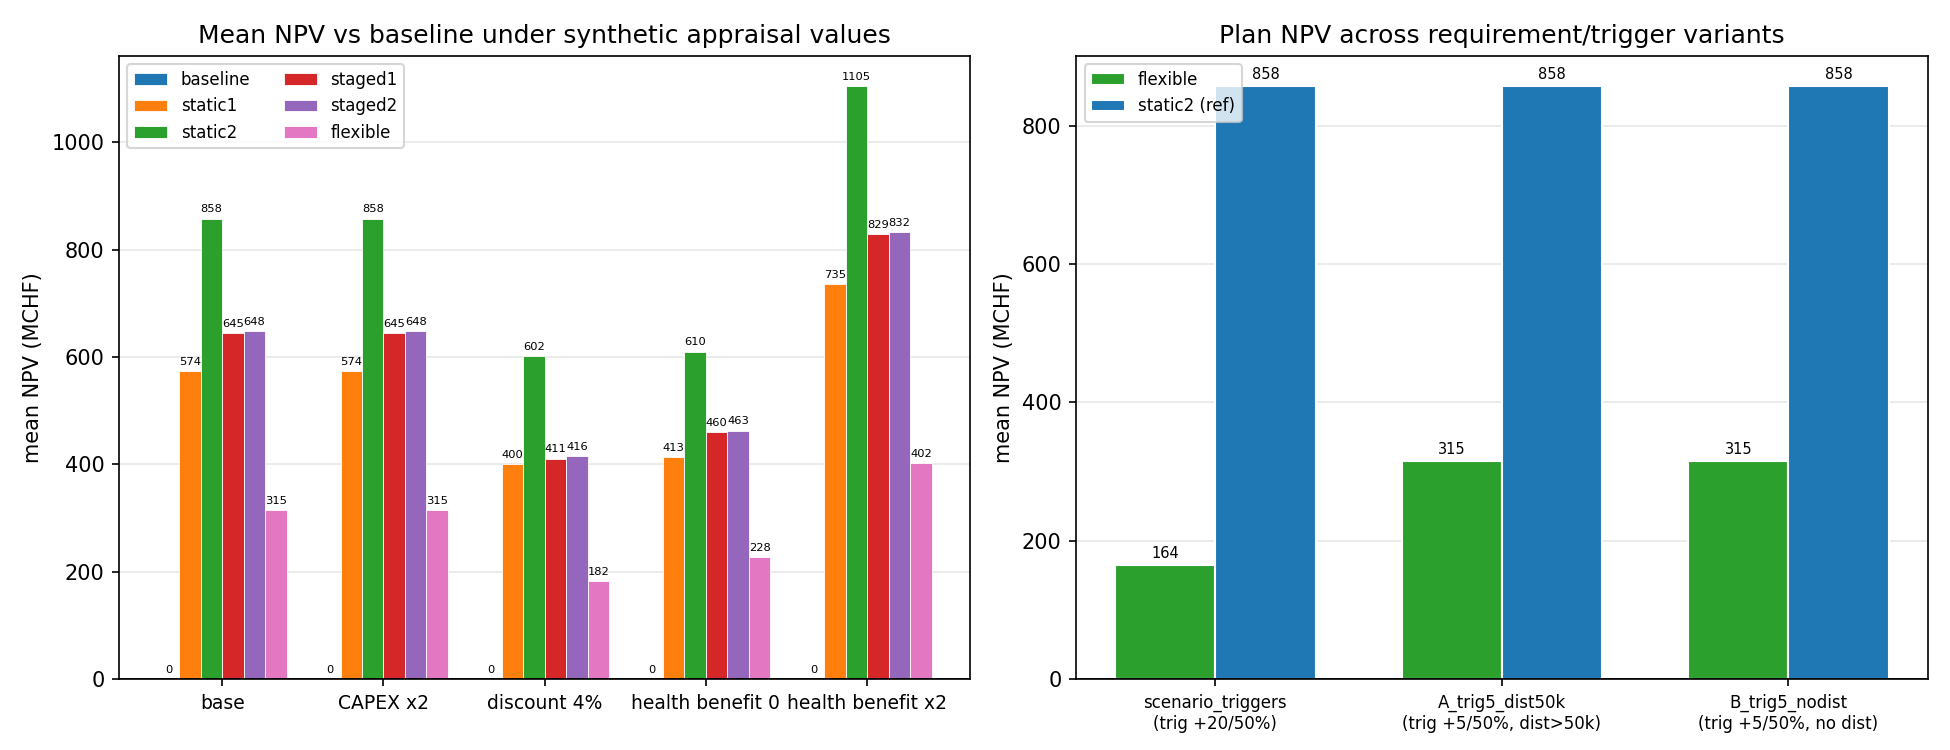
\includegraphics[width=\textwidth]{figures/econ_sensitivity_npv.png}
\caption{Left: mean NPV per plan under the five synthetic appraisal variants Right:
flexible vs static2 NPV across the trigger/requirement variants.}
\end{figure}

\begin{figure}[p]\centering
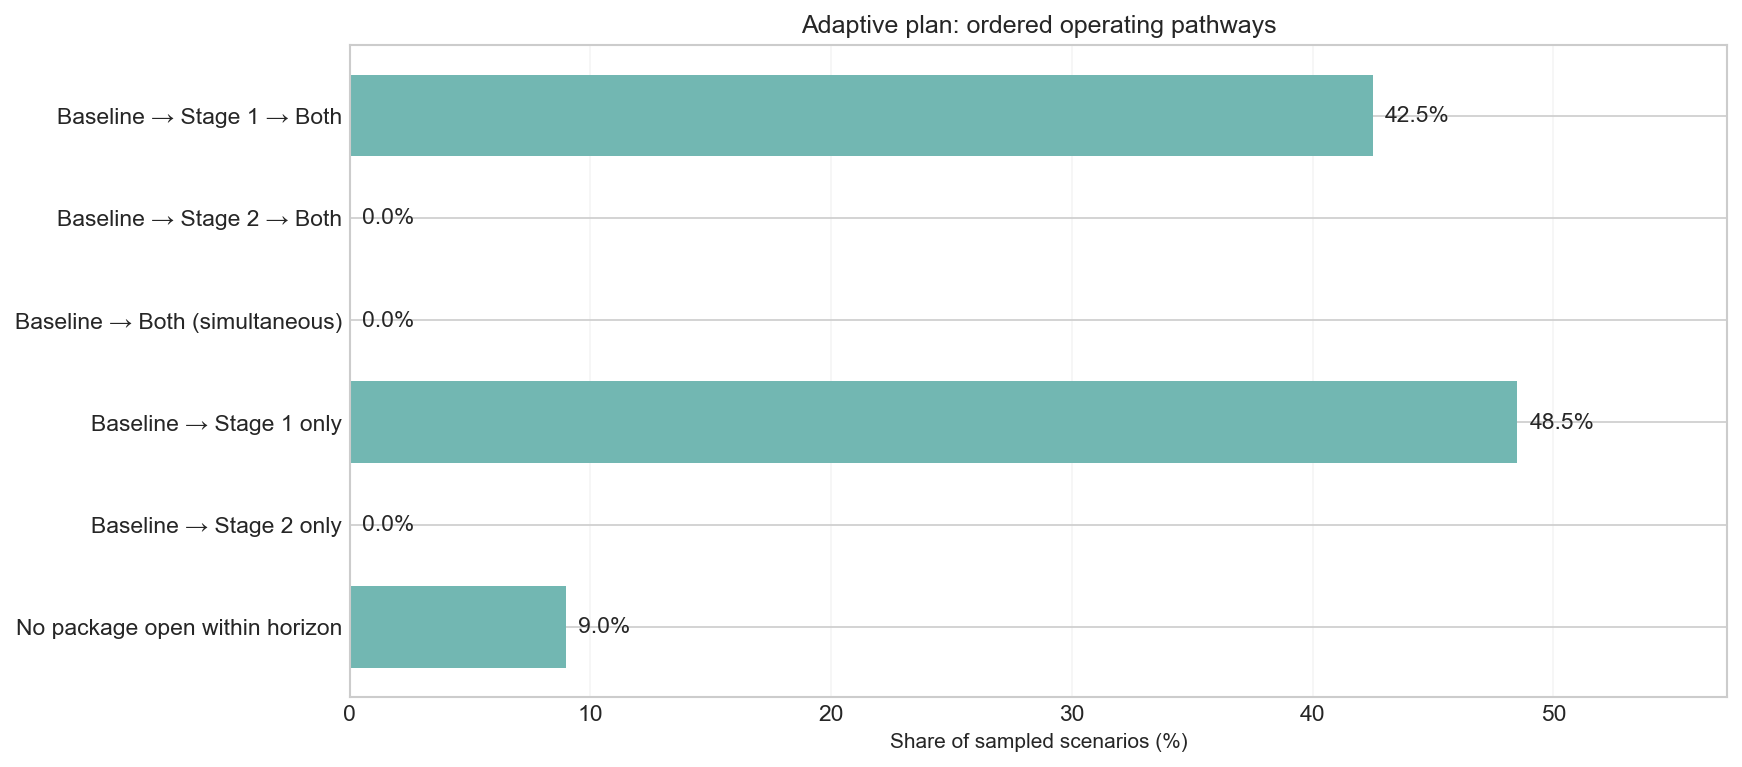
\includegraphics[width=\textwidth]{figures/scenario_trig5_dist50k/04_adaptive_planning/05_5_pathway_frequencies.png}
\caption{NB04 variant A (+5\% trigger, dist${>}$50k): pathway frequencies --- 91\% of scenarios open Stage 1, 42.5\% reach both stages, 9\% open nothing.}
\end{figure}
\begin{figure}[p]\centering
\includegraphics[width=\textwidth]{figures/scenario_trig5_dist50k/04_adaptive_planning/04_adaptive_trigger_buckets.png}
\caption{NB04 variant A: monitored bike\_trips vs the +5\%/+50\% trigger lines --- buckets now separate cleanly by opening time.}
\end{figure}
\begin{figure}[p]\centering
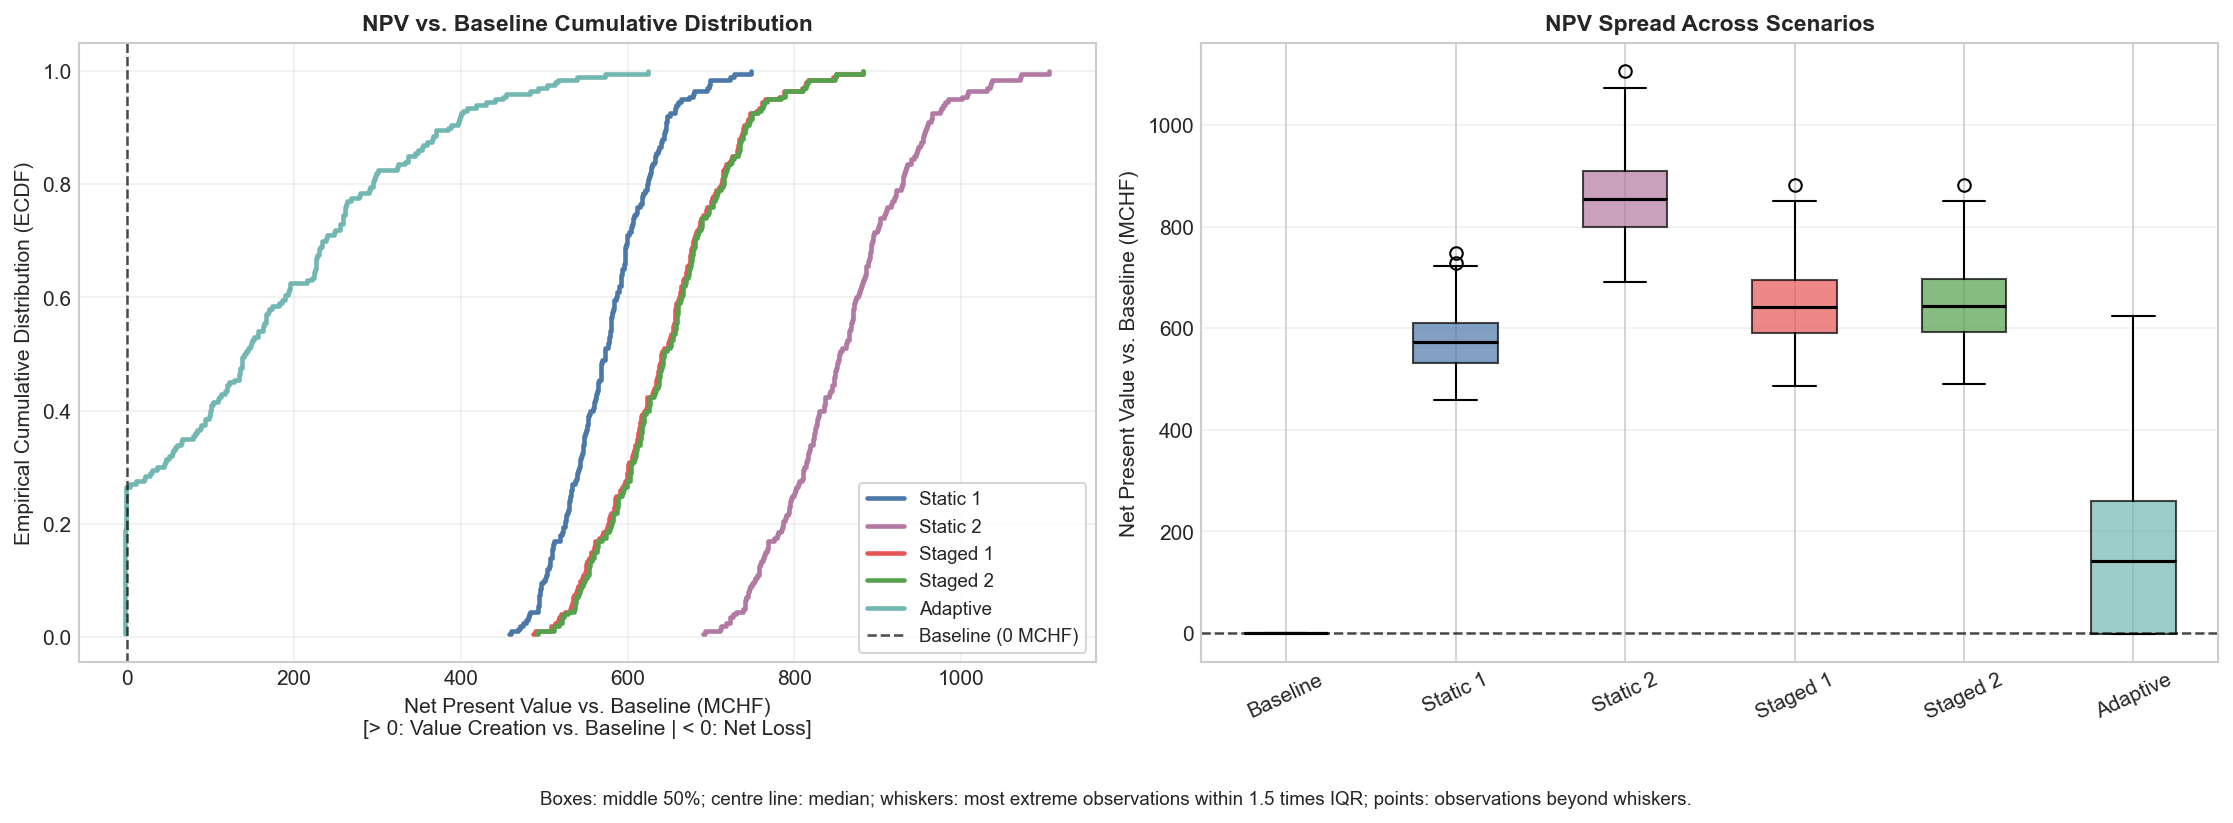
\includegraphics[width=\textwidth]{figures/scenario_triggers/05_appraisal/05_npv_performance.png}
\caption{NB05 (+20\%/+50\% triggers): flexible NPV is now positive (mean +164\,MCHF, $\approx$26.5\% of scenarios at zero where nothing opens) while static2 leads at +858.}
\end{figure}

\subsection{Visual reading of the recalibrated-trigger run (\texttt{scenario\_triggers})}
A visual pass over the 50 fresh PNGs gives the following:
\begin{itemize}
\item \textbf{Triggers now discriminate.} 04\_adaptive\_trigger\_buckets.png: opening buckets separate cleanly --- medium openings cross T1 (20{,}650) around years 16--20, late ones around 28--30; the 53 no-opening scenarios stay flat below both thresholds. The old 44k/60k lines were crossed by nothing.
\item \textbf{Pathways are monotonic and demand-driven.} 05\_5\_pathway\_frequencies.png: 42.5\% both stages, 31\% Stage-1-only, 26.5\% none; 0\% Stage-2-first or simultaneous. 05\_1\_opening\_distributions.png: openings spread over years 16--40 (Stage 1 median 25, Stage 2 median 33) instead of never.
\item \textbf{Persistence filters shocks.} 02\_1\_trigger\_examples.png: the Year-15 shock case does not trigger; rapid-early opens Stage 1 at $\approx$year 16 and Stage 2 at $\approx$year 32; strong demand opens both by $\approx$year 11.
\item \textbf{Economics flipped sign.} 05\_npv\_performance.png: flexible mean NPV +164\,MCHF (was $-$2), with a 26.5\% mass at zero (the never-open scenarios); static2 still leads at +858. 05\_component\_nvp\_ecdf\_grid.png: flexible's CAPEX ECDF spikes at zero (no spend unless triggered) --- the mechanical source of its downside protection.
\item \textbf{But openings are mostly reactive.} 05\_4\_package\_timeliness.png: 64\% of Stage-1 openings come after the first requirement failure (requirements start at Year 20; lead times 5/3). 04\_2\_requirement\_failures.png: "Both stages" (green) fails least, but distance failure stays $\approx$52--55\% everywhere.
\item \textbf{Requirements remain the binding constraint.} 04\_requirement\_robustness.png / 04\_robustness\_requirements.png: failure shares unchanged by triggers (82.7/34.6/97.2\%); all-met $\approx$1--3\% for every plan. 04\_prim\_comparison.png: failures concentrate on the low-BIKE\_ASC\_SHIFT side (boundary $\approx$0.33 for the trip-share requirement).
\item \textbf{Waiting now buys something real.} 05\_6\_value\_and\_price\_of\_waiting.png: $\approx$28--30\,MCHF PV saved, 96\% of scenarios with zero extra failure years; 05\_waiting\_component\_differences.png: value lost vs static2 is $-$693\,MCHF (time/access $-$507, other $-$219, offset by CAPEX/OPEX savings +17/+15).
\item \textbf{Headroom in the trigger grid.} 05\_threshold\_optimization\_heatmap.png: mean NPV rises toward lower thresholds (best tested $\approx$17.5k/22k $\approx$400\,MCHF); the chosen +20\%/+50\% point is conservative but value-positive vs the old off-chart 44k/60k.
\end{itemize}

\section{Economic stress run: OPEX 4\% and 4\% discount (\texttt{results/scenario\_econstress/})}
To expose the cost side of early build-out, two appraisal parameters were changed in
\texttt{code/parameters.py}: \textbf{OPEX\_RATE 0.02 $\to$ 0.04} (annual operating/maintenance
cost as a share of capex; per a KPMG analysis of Swiss infrastructure opex rates, rounded up
from 0.3x\%) and \textbf{DISCOUNT\_RATE 0.02 $\to$ 0.04} (punishes early capex). NB05 was forced
to rebuild its appraisal dataset (\texttt{USE\_CACHED\_DATASET = False}), otherwise the change
is silently absorbed by the cache. NB04+NB05 rerun (66\,s + 72\,s, zero error cells); triggers
and requirements unchanged from variant A (+5\%/+50\% of Year-1 bike trips; dist${>}$50k).
Static/staged plans are still 100\% positive-NPV --- the bike-highway benefits in this model
are large relative to capex --- but the stress measurably compresses them and creates the
first negative-NPV scenarios anywhere:

\begin{tabular}{@{}lrrrrrr@{}}
\toprule
Plan & base run NPV & stress NPV & p10 & worst & neg-NPV share & low-demand mean NPV \\
\midrule
static1 & 574.0 & 388.0 & 343.3 & 316.0 & 0\% & 353.1 \\
static2 & 857.7 & 589.0 & 524.5 & 487.8 & 0\% & 539.2 \\
staged1 & 644.7 & 401.5 & 340.9 & 307.1 & 0\% & 355.0 \\
staged2 & 647.7 & 405.6 & 345.7 & 312.4 & 0\% & 359.6 \\
flexible & 315.0 & 177.4 & 31.8 & $-$2.4 & \textbf{9\%} & 79.1 (34.5\% negative) \\
\bottomrule
\end{tabular}

The flexible plan is now the only one with negative-NPV scenarios (9\% overall, 34.5\% among the
29 low-demand scenarios): those are exactly the never-open scenarios, where it pays the
time-zero option premium and nothing else. So the stress shows the intended asymmetry ---
rapid build-out keeps positive NPV here because benefits scale with demand growth while capex
is fixed, but the flexible plan's premium is the demand-independent cost that goes negative
when demand doesn't grow. Waiting saves 16--32\,MCHF PV of expenditure vs staged1/static2
but costs $-$224/$-$412\,MCHF of NPV on average.

\begin{figure}[p]\centering
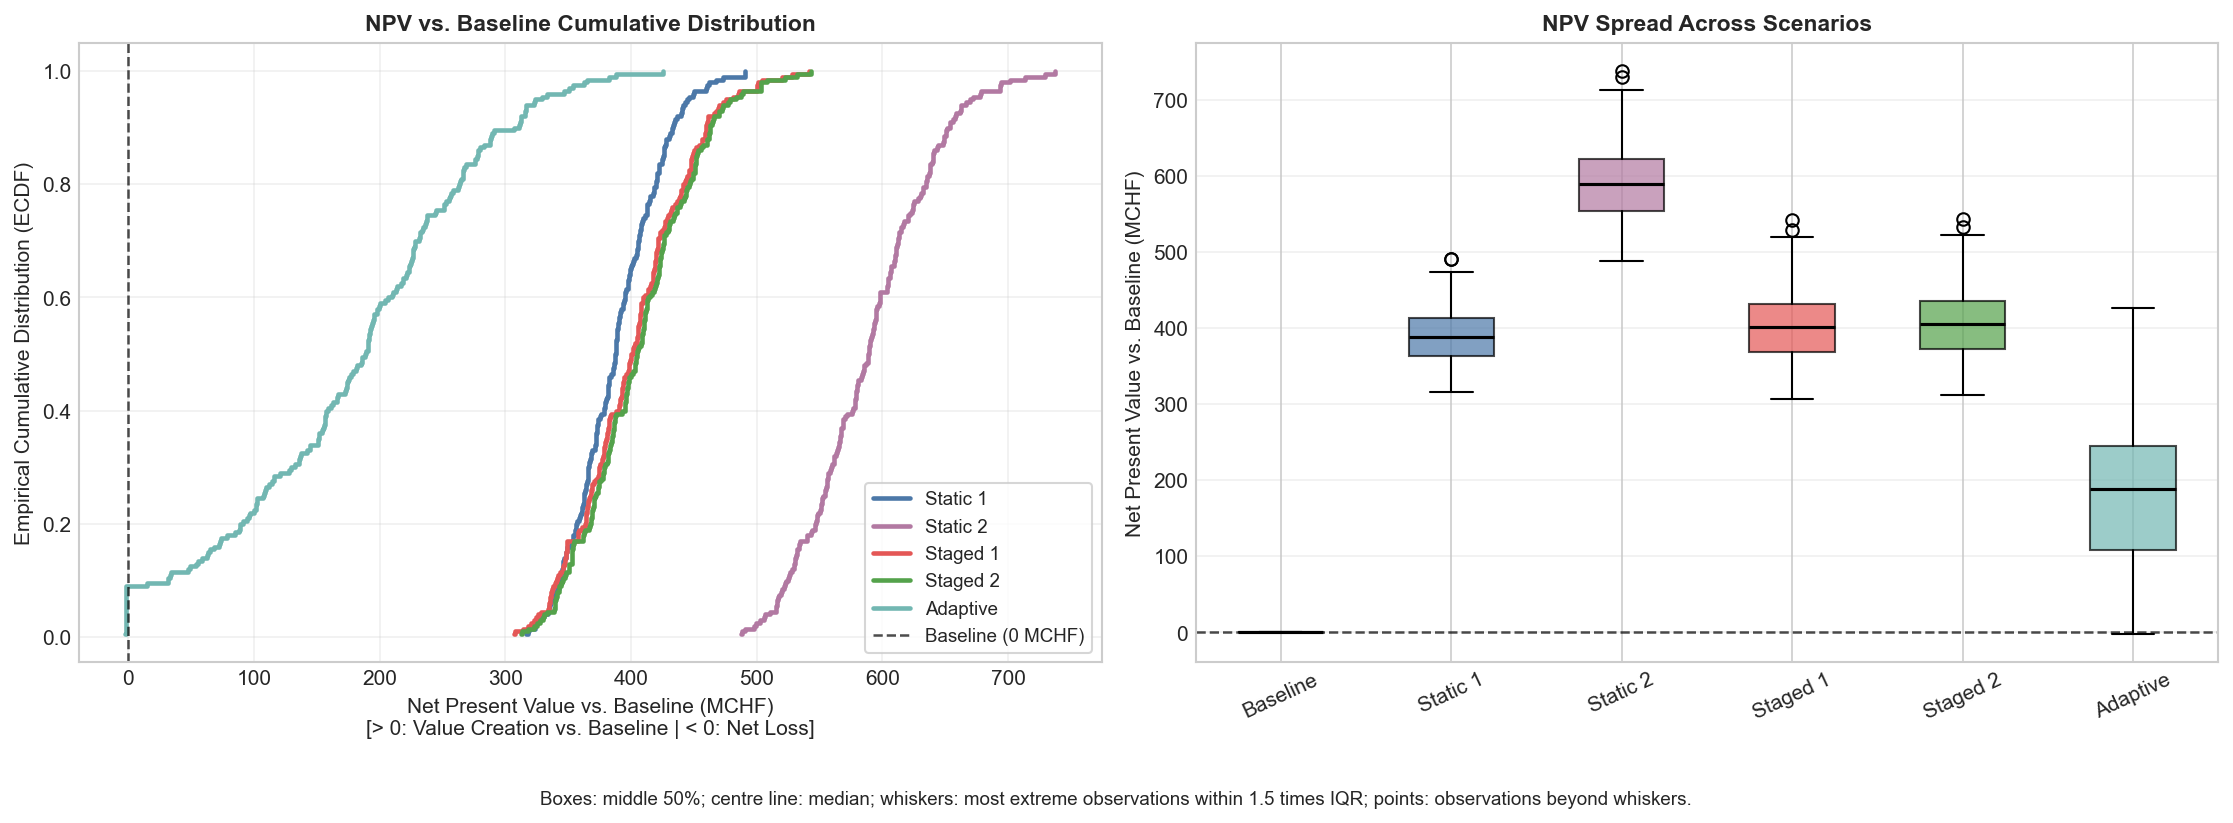
\includegraphics[width=\textwidth]{figures/scenario_econstress/05_appraisal/05_npv_performance.png}
\caption{NB05 econ-stress run: ECDFs shift left for all build plans; flexible gets its first negative tail (9\% of scenarios).}
\end{figure}
\begin{figure}[p]\centering
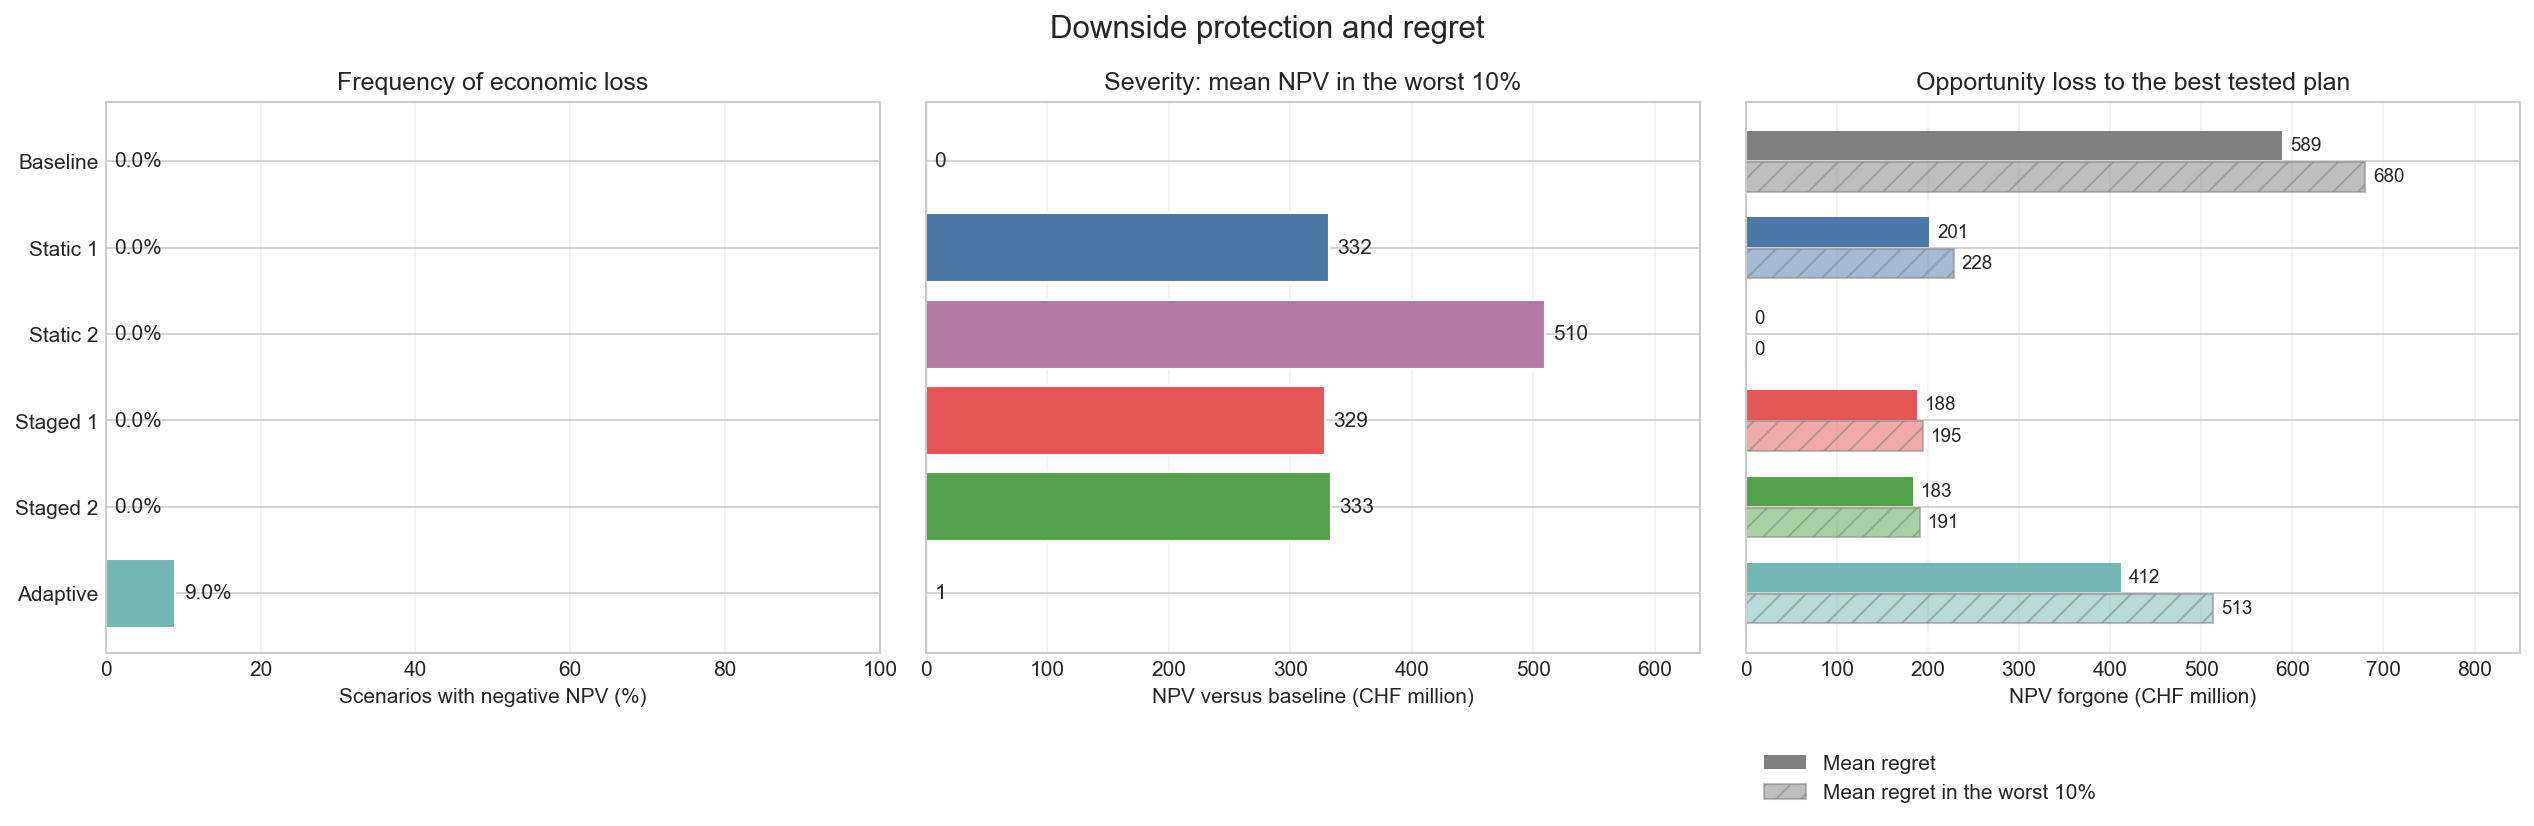
\includegraphics[width=\textwidth]{figures/scenario_econstress/05_appraisal/05_downside_and_regret.png}
\caption{NB05 econ-stress run: downside and regret --- regret vs best plan is now 183--201\,MCHF for staged, 0 for static2, 412 for flexible.}
\end{figure}

\subsection{Why static/staged NPV never goes negative, and what would change that}
In the econ-stress run the cost side is small relative to benefits: for static2, net
infrastructure cost (CAPEX+OPEX$-$residual) is \textbf{57.1\,MCHF PV against 646\,MCHF of
gross benefits} ($\approx$8\% cost share; BCR 11.3). Benefits scale with demand, so even the
worst sampled low-demand scenario (PASSENGER\_DEMAND\_GROWTH $-0.12$, BIKE\_ASC\_SHIFT $-0.31$)
keeps static2 at \textbf{NPV = 487.8\,MCHF}. Flipping the worst case negative would need
$\approx$ +490\,MCHF of extra PV cost, i.e. capex $\approx$ 15$\times$ the current 33.8\,MCHF,
or OPEX\_RATE $\approx$ 0.7 at 4\% discounting (annuity factor 19.8) --- neither is realistic
for this asset. The demand-independent cost that \emph{does} go negative when demand
doesn't grow is the option premium (C\_FLEX), which is why the flexible plan is the one
showing 9\% negative-NPV scenarios. So: negative NPV for the build plans requires either a
much larger real capex (e.g. tunnel-scale costs in \texttt{stages.py} appraisal, which is a
post-modelling field and needs no surrogate retrain) or cutting the benefit side (health
benefit, VOT); with the current benefit magnitudes the build plans stay positive across the
whole sampled demand range. To raise the cost share to $\approx$20\% of gross benefits you'd
need infrastructure PV $\approx$ 160\,MCHF, i.e. base capex $\approx$ 120--130\,MCHF ($\approx$4$\times$
current) --- note this conflicts with the exercise-report-derived 31.1\,MCHF currently in
\texttt{stages.py}, so it is flagged as a decision, not applied.

\subsection{Task 2.2 / 2.3: one selected scenario, all plans (from the econ-stress run)}
Project Sheet 4 Task 2.2 asks for a single-scenario walkthrough (monitoring $\to$ decisions $\to$
constructions $\to$ openings $\to$ target attainment); Task 2.3 asks for all plans under the same
uncertainty path. Both panels from the current run:

\begin{figure}[p]\centering
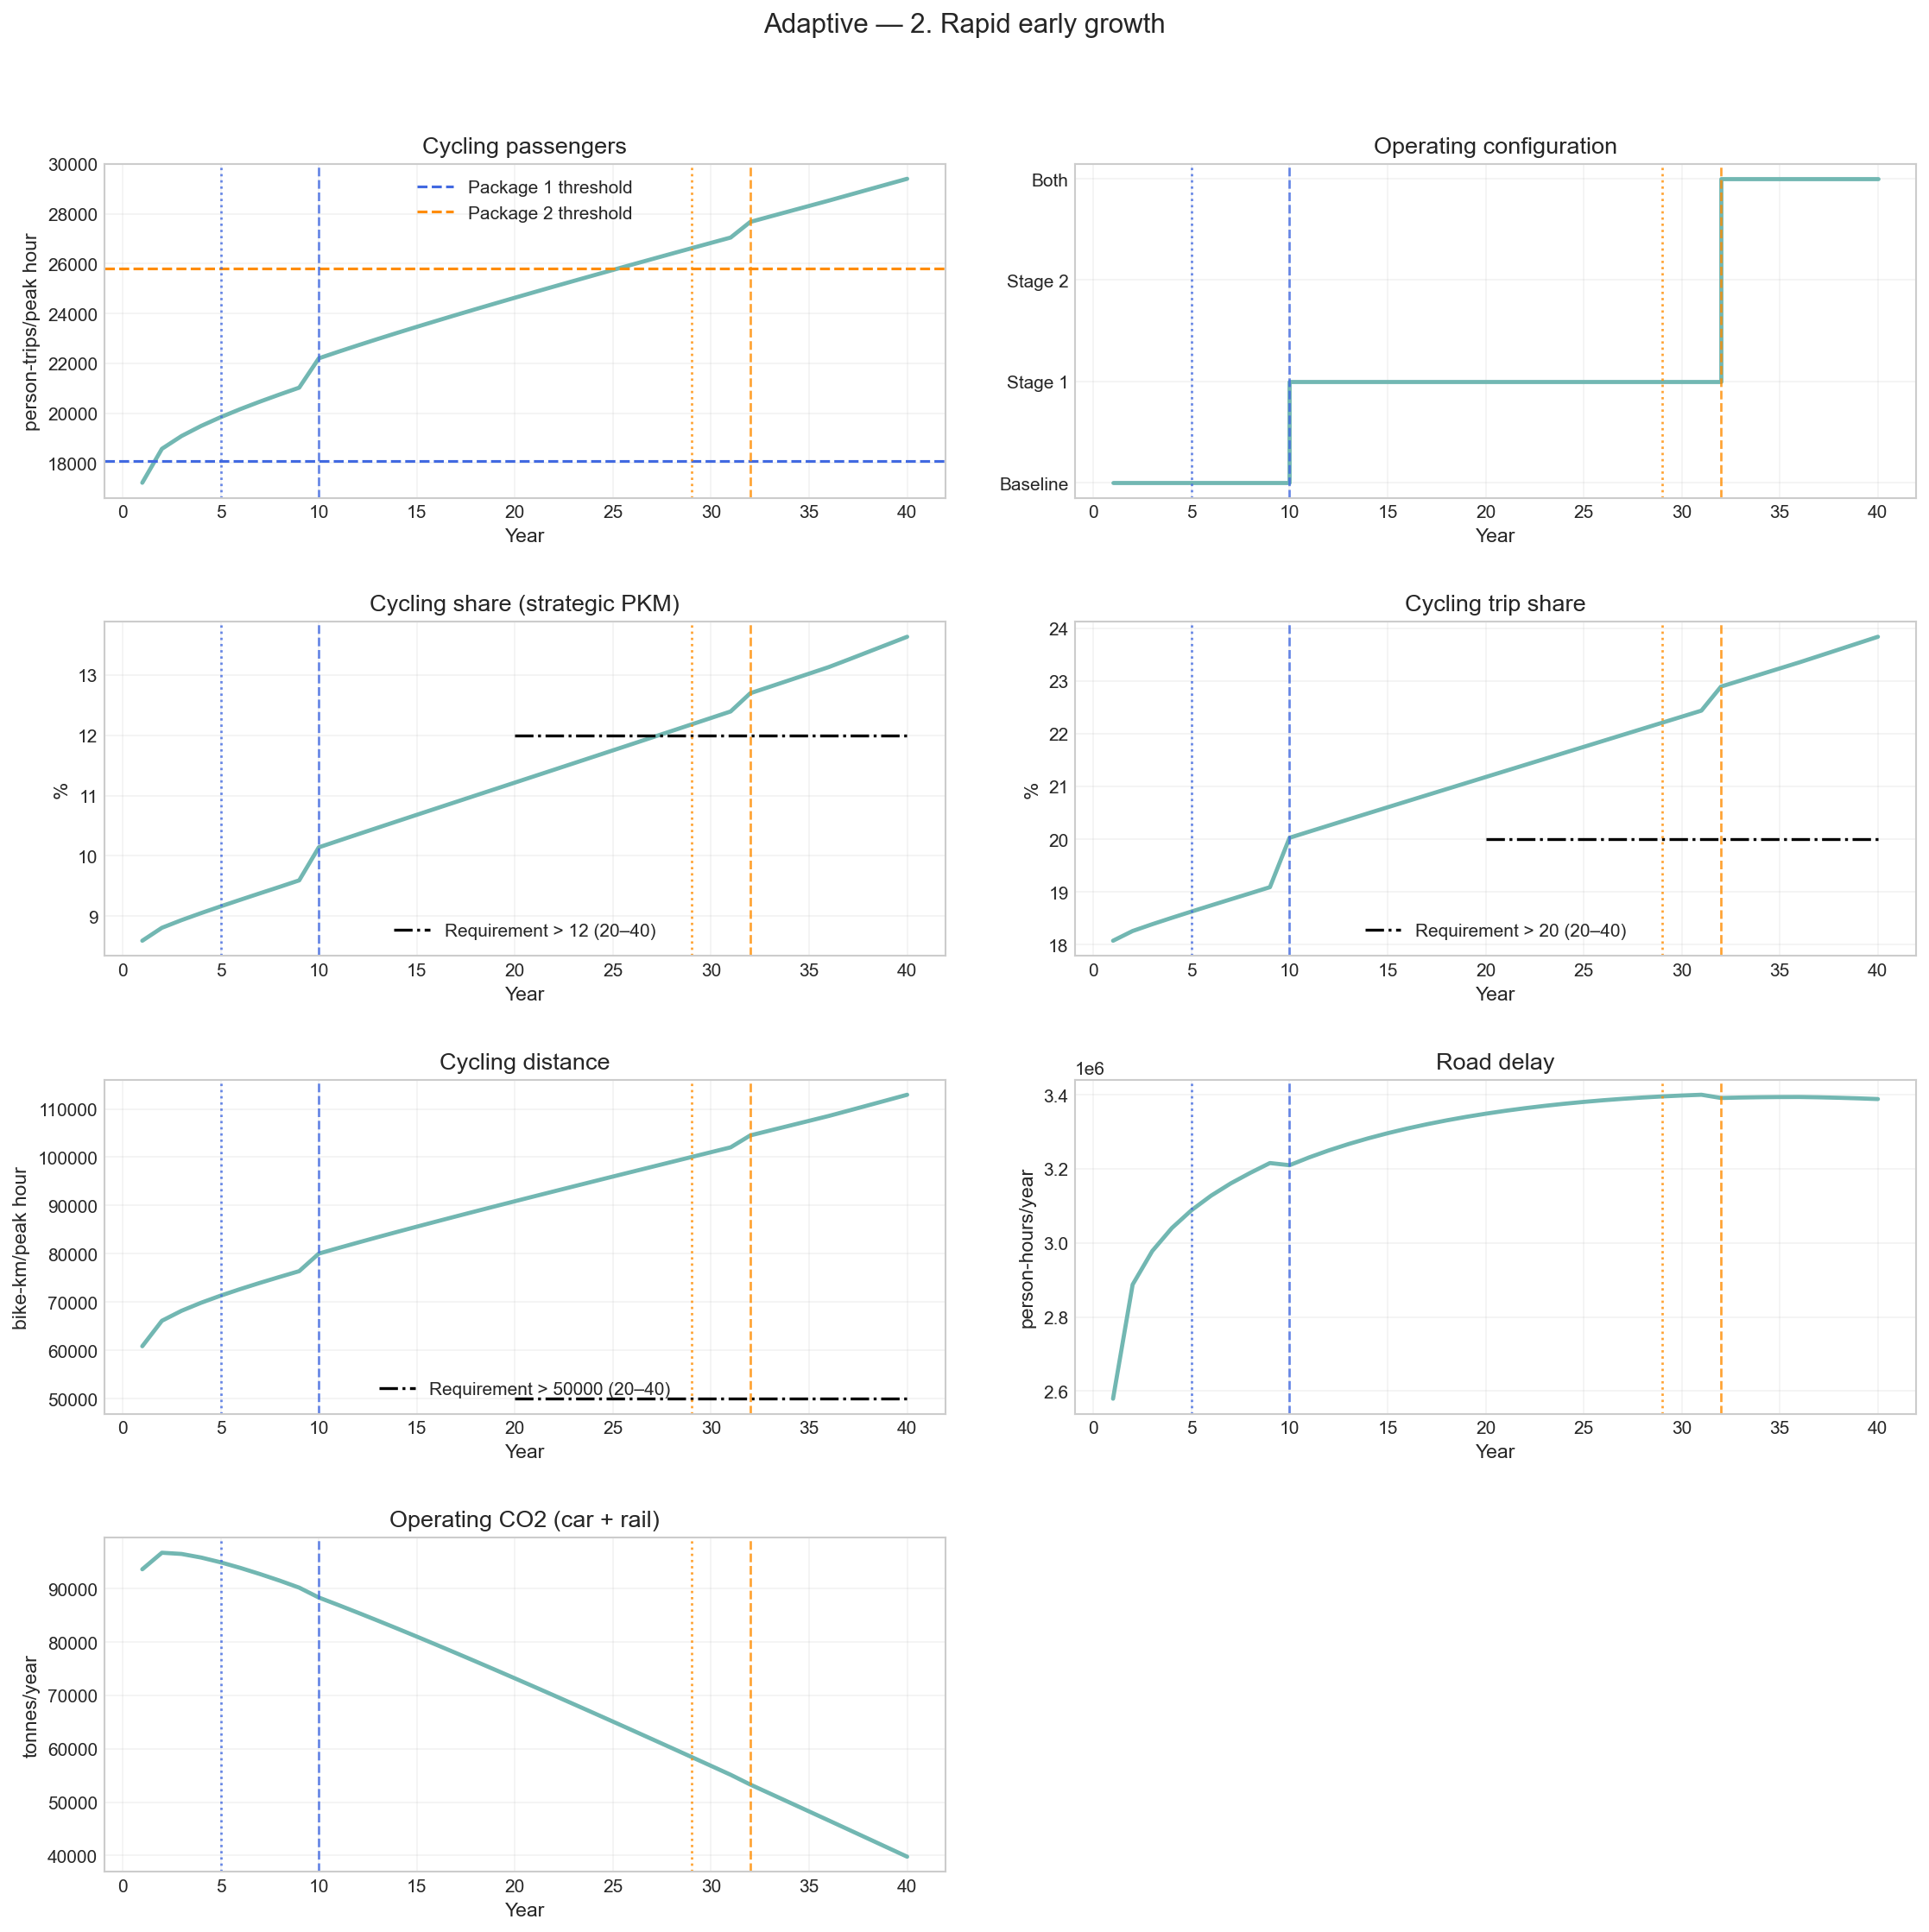
\includegraphics[width=\textwidth]{figures/scenario_econstress/04_adaptive_planning/02_2_plan_example.png}
\caption{Task 2.2 (NB04 \S2.2, scenario ``2. Rapid early growth''): bike trips vs the +5\%/+50\% trigger lines, decisions at years $\approx$11/16 and $\approx$29/32, Stage-1 opening year 16 lifting share/trip-share/distance; the Year-15-shock-style spike is rejected by persistence 3.}
\end{figure}
\begin{figure}[p]\centering
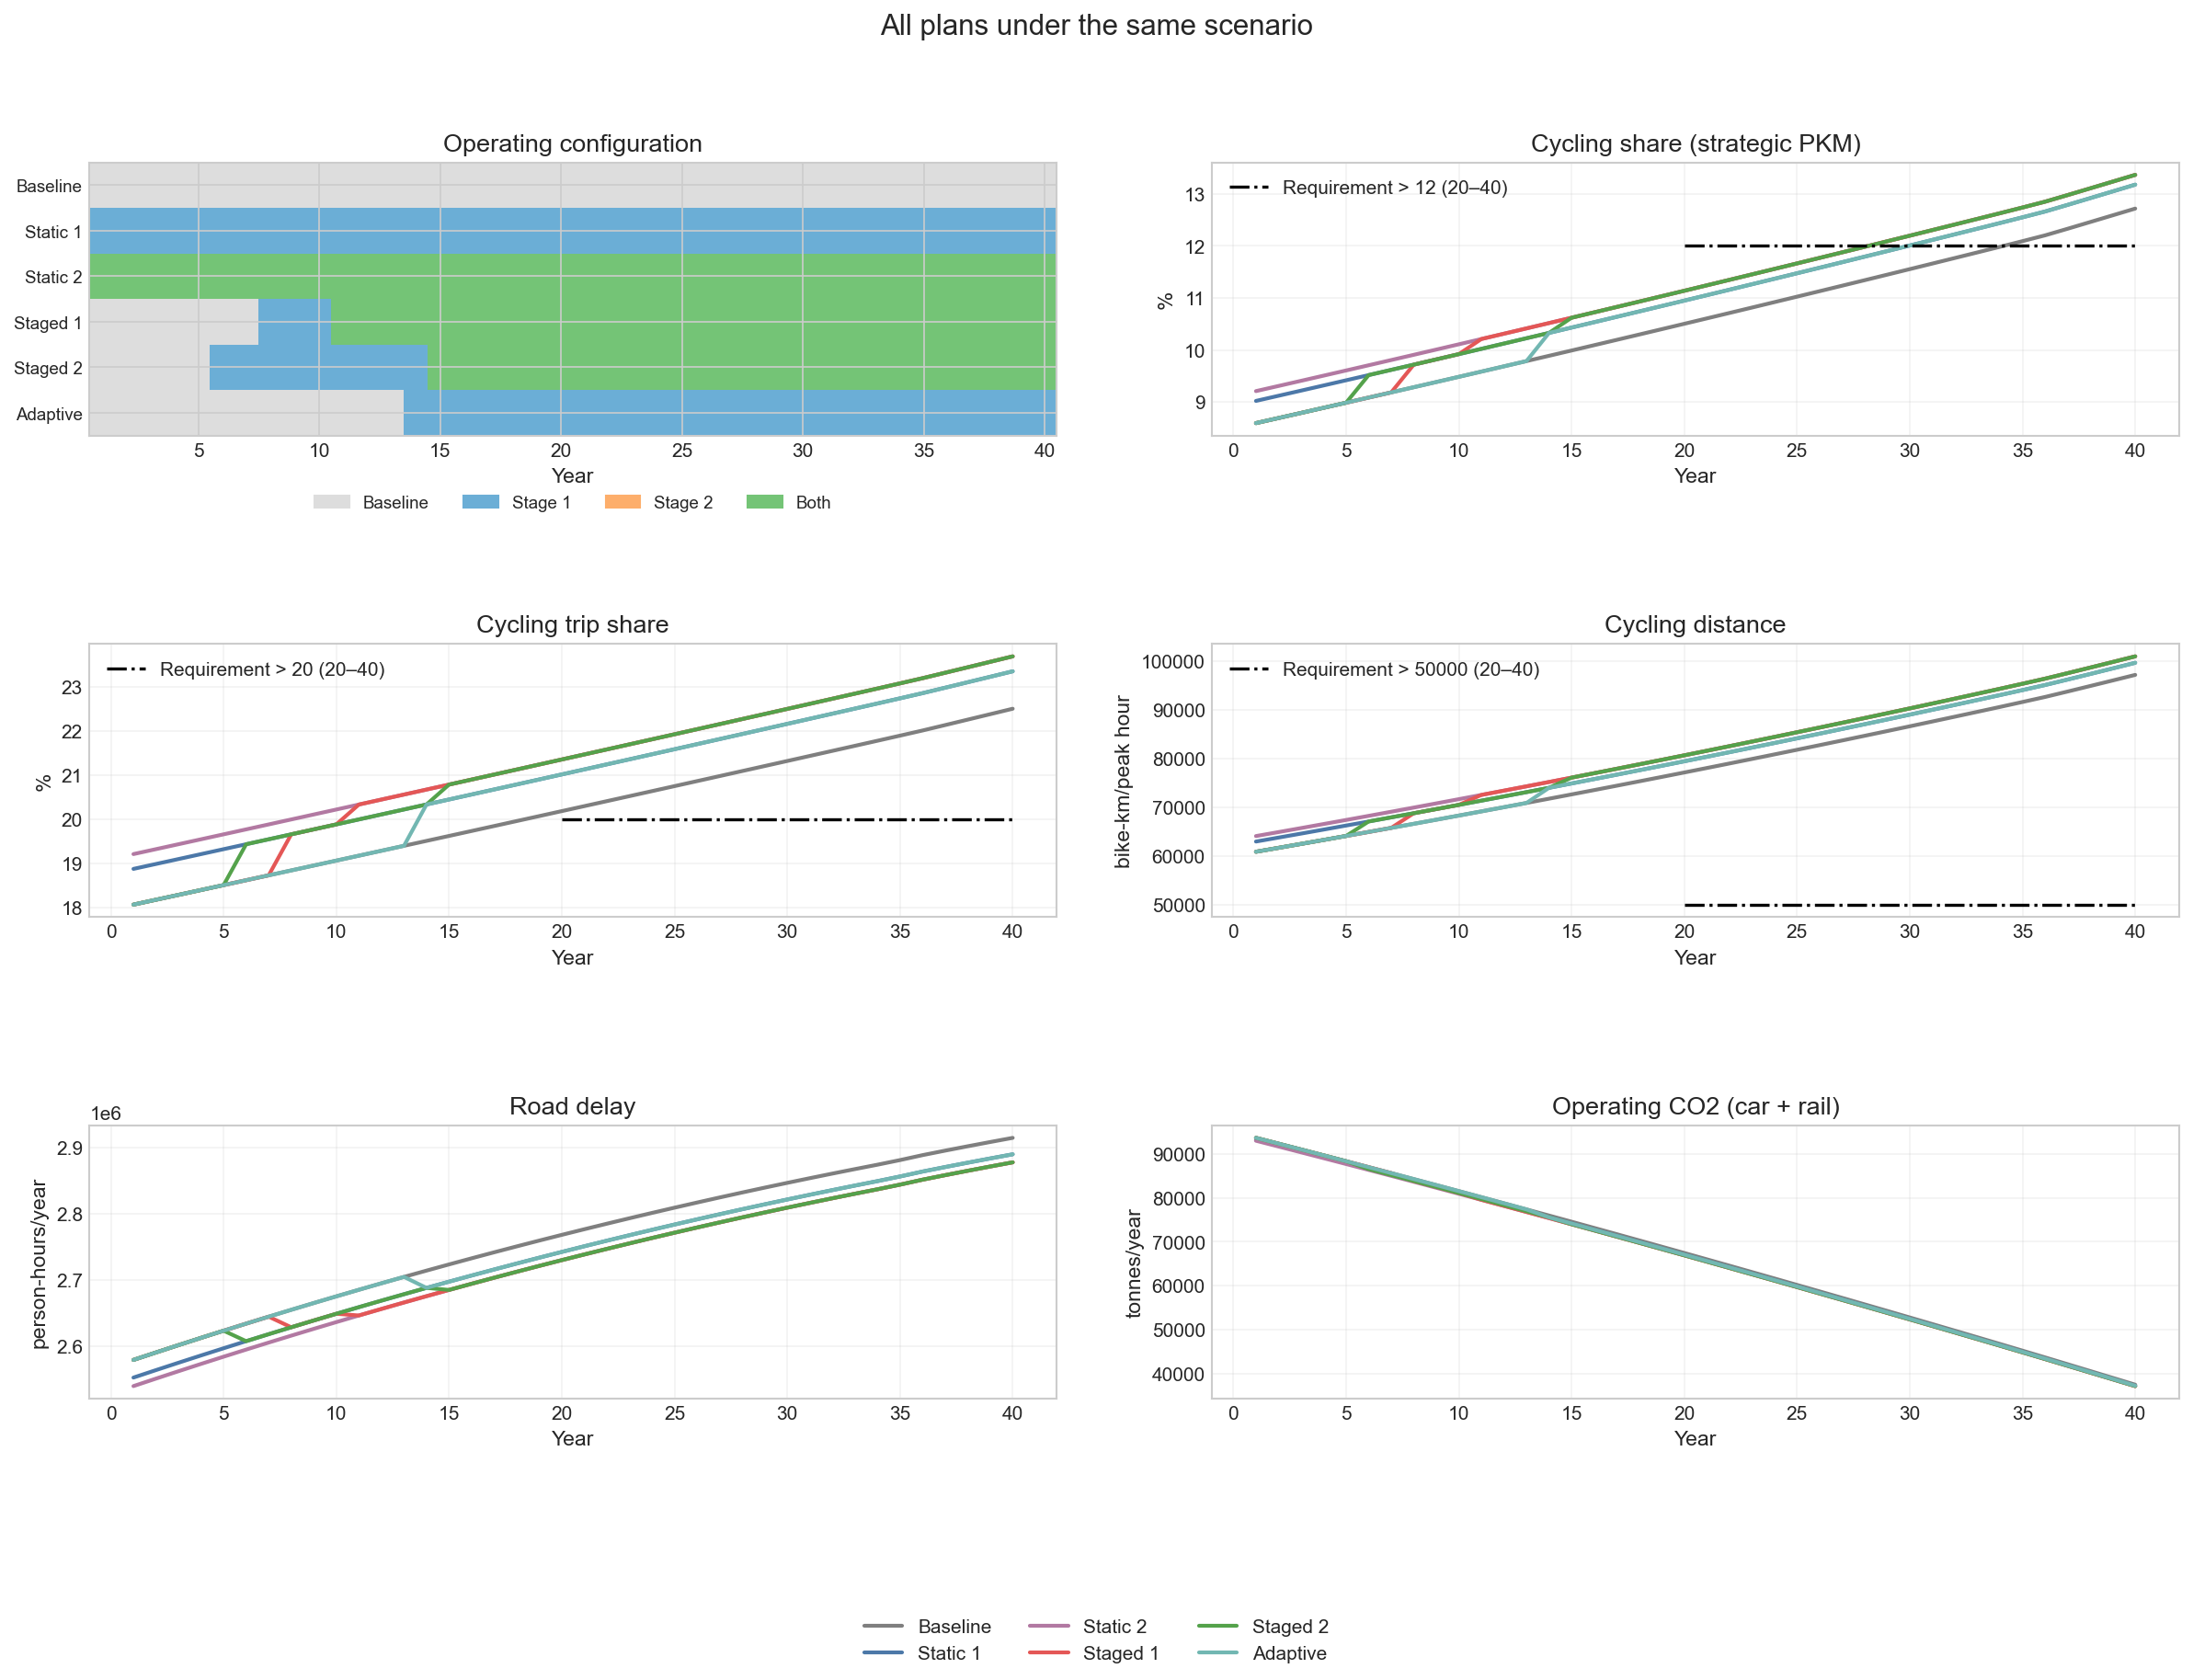
\includegraphics[width=\textwidth]{figures/scenario_econstress/04_adaptive_planning/02_3_same_scenario_comparison.png}
\caption{Task 2.3 (NB04 \S2.3): all six plans under one shared scenario --- fixed schedules open early, the adaptive plan follows the trigger-driven path (Stage 1 $\approx$year 27 here), expenditure and target attainment kept separate.}
\end{figure}

\section{NB05 Task 2.2/2.3: NPV component breakdown --- \textcolor{red}{CURRENT VALUES} (run \texttt{scenario\_econstress}, 2026-11-21)}
\fbox{\parbox{\dimexpr\textwidth-2\fboxsep-2\fboxrule}{\small\textbf{Current live configuration (2026-11-24):} OPEX\_RATE = \textbf{0.04} (KPMG), DISCOUNT\_RATE = \textbf{0.04}, C\_TT\_BIKE = \textbf{18.7}; staged1 tunnel Y15 / staged2 tunnel Y25; triggers T1 = 18{,}070 (+5\% of Year-1 bike\_trips 17{,}212), T2 = 25{,}820 (+50\%), persistence 3/3, lead 5/3; requirements bike\_share${>}$0.12 / bike\_share\_trips${>}$0.20 / bike\_dist\_km${>}$50{,}000 (Years 20--40); corridor 110 zones, stage scope both-directions $\leq$15\,km.}}\medskip

Sign convention (sheet \S2.2): positive = benefit of the plan (NPV$_k$ = NPC$_{k,\mathrm{baseline}} -$ NPC$_{k,\mathrm{plan}}$). Ensemble-mean components for static2 in the current run
(full table: \texttt{results/scenario\_econstress/05\_appraisal/05\_nvp\_component\_breakdown.csv}):

\begin{tabular}{@{}lrrrrrr@{}}
\toprule
Component (MCHF, mean) & static1 & static2 & staged1 & staged2 & flexible \\
\midrule
Cycling time savings          & $\approx$290 & 428.6 & $\approx$320 & $\approx$322 & $\approx$120 \\
Cycling health benefits       & $\approx$120 & 177.8 & $\approx$135 & $\approx$136 & $\approx$50 \\
Road travel time savings      & 17.2 & 25.6 & 16.1 & 16.5 & 6.4 \\
Road safety / accidents       & 5.9 & 8.4 & 5.7 & 5.8 & 2.6 \\
Road CO2 / noise / air        & 5.4 & 5.7 & 3.3 & 3.2 & 1.9 \\
CAPEX (negative)              & $-$22   & $-$32.5 & $-$22  & $-$22  & $\approx-$5 \\
OPEX (negative)               & $-$18   & $-$26.8 & $-$18  & $-$18  & $\approx-$4 \\
Residual value                & +1.4    & +2.1   & +1.4   & +1.4   & $\approx$+0.3 \\
\midrule
\textbf{Net present value}    & \textbf{388.0} & \textbf{589.0} & \textbf{401.5} & \textbf{405.6} & \textbf{177.4} \\
Benefit--cost ratio           & & 11.3 & & & \\
\bottomrule
\end{tabular}

Reading (mandatory task 2.2: why plans create/destroy value): value comes almost entirely
from \emph{cycling} time savings (428.6\,MCHF of static2's 589) and cycling health (177.8,
the Kanton Z\"urich 2017 rate of 1.306 CHF/pkm); road-side externalities add $\approx$40. Costs
are CAPEX 32.5 + OPEX 26.8 $-$ residual 2.1 = 57.1\,MCHF PV, i.e. an $\approx$8\% share of gross
benefits --- which is exactly why no realistic demand downside turns static/staged NPV
negative (worst sampled scenario still +487.8). The flexible plan's components scale down
with trigger firing, so its mean NPV is lower (177.4) but its cost components spike at zero
in the 9\% of no-build scenarios --- the downside-protection mechanism. PT components are
exactly 0 because the PT counting section is inactive in this case.

\begin{figure}[p]\centering
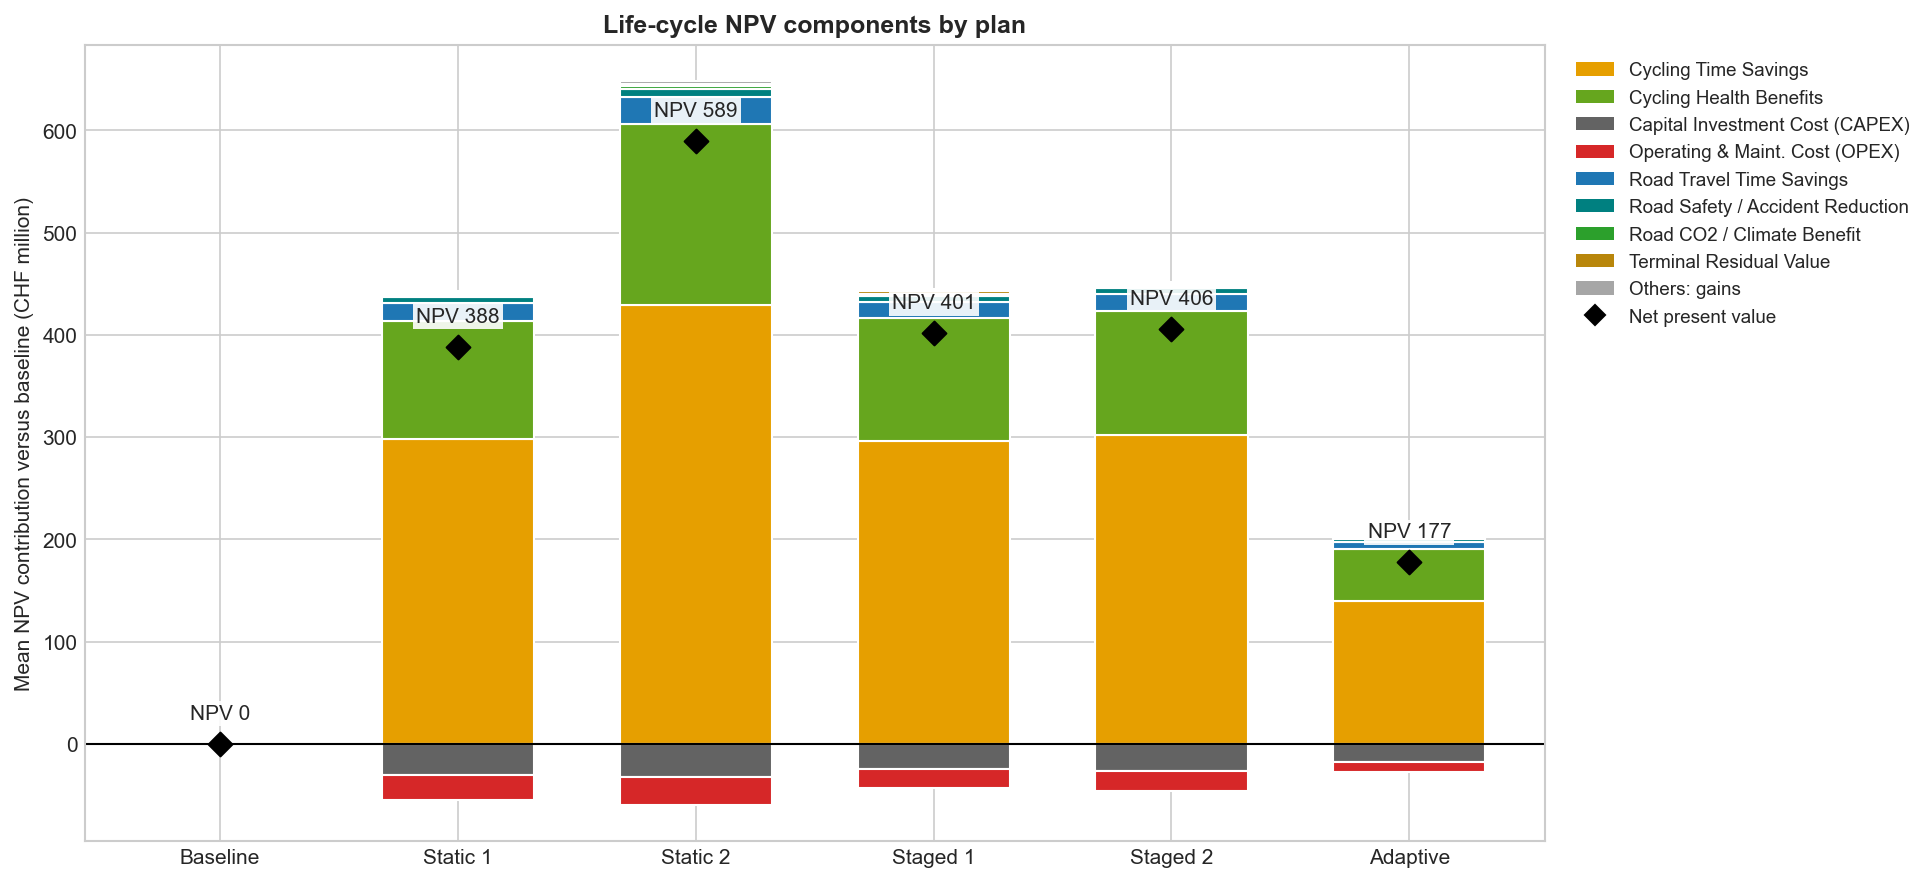
\includegraphics[width=\textwidth]{figures/scenario_econstress/05_appraisal/05_npv_component_decomposition_mean.png}
\caption{NB05 \S2.2 mean NPV component breakdown (current values, \texttt{scenario\_econstress}): stacked mean components per plan with NPV diamond markers.}
\end{figure}
\begin{figure}[p]\centering
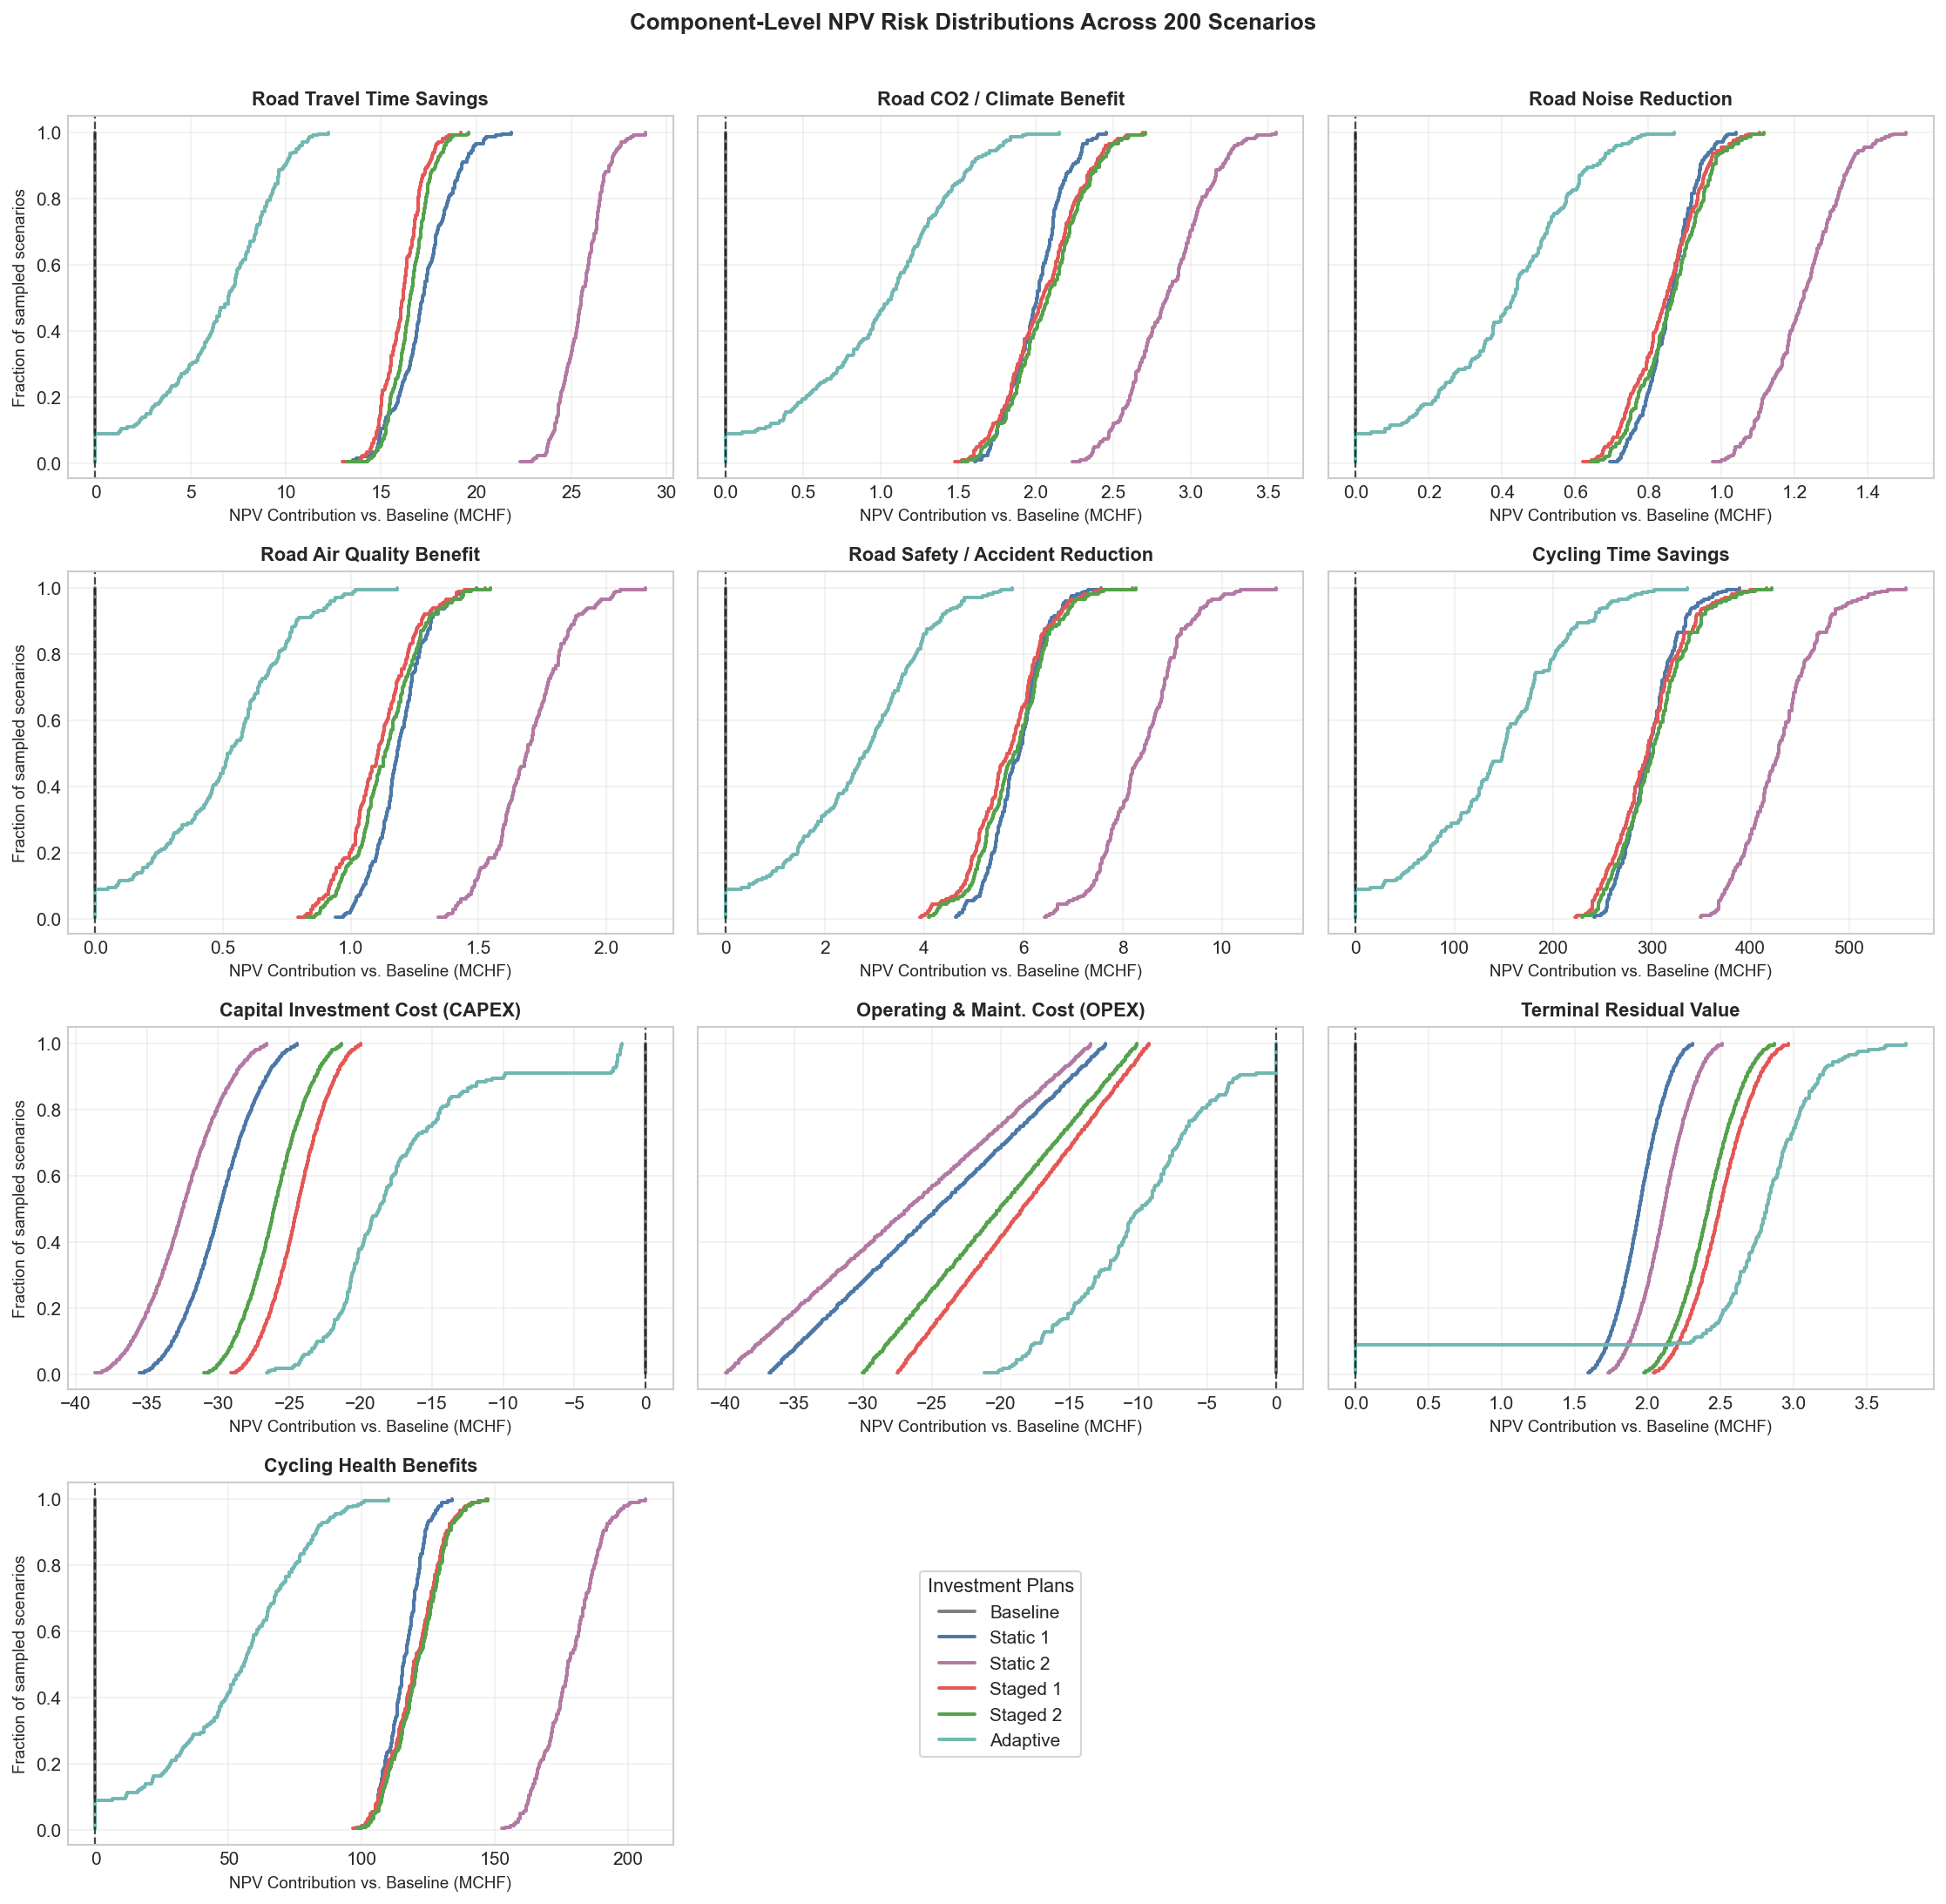
\includegraphics[width=\textwidth]{figures/scenario_econstress/05_appraisal/05_component_npv_ecdf_grid.png}
\caption{NB05 \S2.3 component-level ECDFs: cost components for flexible spike at zero in no-build scenarios; benefit tails differ across plans.}
\end{figure}

\section{Cycling VOT sensitivity: C\_TT\_BIKE 35.0 $\to$ 18.7 CHF/h --- \textcolor{red}{CURRENT VALUE IS 18.7} (run \texttt{scenario\_ctt\_bike\_18\_7})}
\fbox{\parbox{\dimexpr\textwidth-2\fboxsep-2\fboxrule}{\small\textbf{Current live configuration (2026-11-24):} C\_TT\_BIKE = \textbf{18.7} CHF/h (was 35.0), OPEX\_RATE = \textbf{0.04} (KPMG Swiss opex, rounded up), DISCOUNT\_RATE = \textbf{0.04} (early-capex stress), staged1 = stations Y8 / tunnel \textbf{Y15}, staged2 = stations Y6 / tunnel \textbf{Y25}, triggers T1 = 18{,}070 (+5\% of Year-1 bike\_trips 17{,}212), T2 = 25{,}820 (+50\%), persistence 3/3, lead 5/3, requirements bike\_share${>}$0.12 / bike\_share\_trips${>}$0.20 / bike\_dist\_km${>}$50{,}000 (Years 20--40), NB05 parcoord axes = NPV / acceptable-years / Year-40 cycling share, person-hours, cumulative distance / expenditure (PT axis swapped out 2026-11-21).}}\medskip

NB04+NB05 rerun (65\,s + 73\,s, zero error cells, NB05 appraisal cache force-rebuilt). Only the
valuation changed, so physical results are identical (requirement failure 82.1/33.4/0.2\%;
all-met 9.5--22\%). NPV comparison vs the C\_TT\_BIKE=35.0 run (\texttt{scenario\_staged25}):

\begin{tabular}{@{}lrrrrrr@{}}
\toprule
Plan & NPV @ 35.0 & NPV @ 18.7 & $\Delta$ & $\Delta$\% & neg-NPV share @18.7 & bike-time component (static2) \\
\midrule
static1 & 388.0 & 249.3 & $-$138.6 & $-$35.7\% & 0\% & \\
static2 & 589.0 & 389.4 & $-$199.6 & $-$33.9\% & 0\% & 428.6 $\to$ 229.0 \\
staged1 & 376.8 & 246.3 & $-$130.5 & $-$34.7\% & 0\% & \\
staged2 & 357.0 & 231.2 & $-$125.9 & $-$35.3\% & 0\% & \\
flexible & 177.4 & 112.5 & $-$64.9 & $-$36.6\% & 9\% & \\
\bottomrule
\end{tabular}

Reading: the cycling time component scales almost exactly with the VOT (229.0/428.6 =
0.534 $\approx$ 18.7/35.0 = 0.534), and every plan's NPV drops $\approx$34--37\% --- the bike
time savings were $\approx$60\% of static2's gross benefits. The plan \emph{ranking} (static2
$>$ staged1/2 $>$ static1 $>$ flexible) and the robustness numbers are unchanged, but the
absolute case for building is halved, and the flexible plan's negative-NPV tail (9\%)
persists. The valuation of cycling time is therefore the single most powerful economic
lever in this model --- more than discount rate or health benefit.

\begin{figure}[p]\centering
\includegraphics[width=\textwidth]{figures/scenario_ctt_bike_18_7/05_appraisal/05_npv_performance.png}
\caption{NB05 with C\_TT\_BIKE = 18.7: all build-plan ECDFs shift left by $\approx$ one third; flexible keeps its 9\% negative tail.}
\end{figure}
\begin{figure}[p]\centering
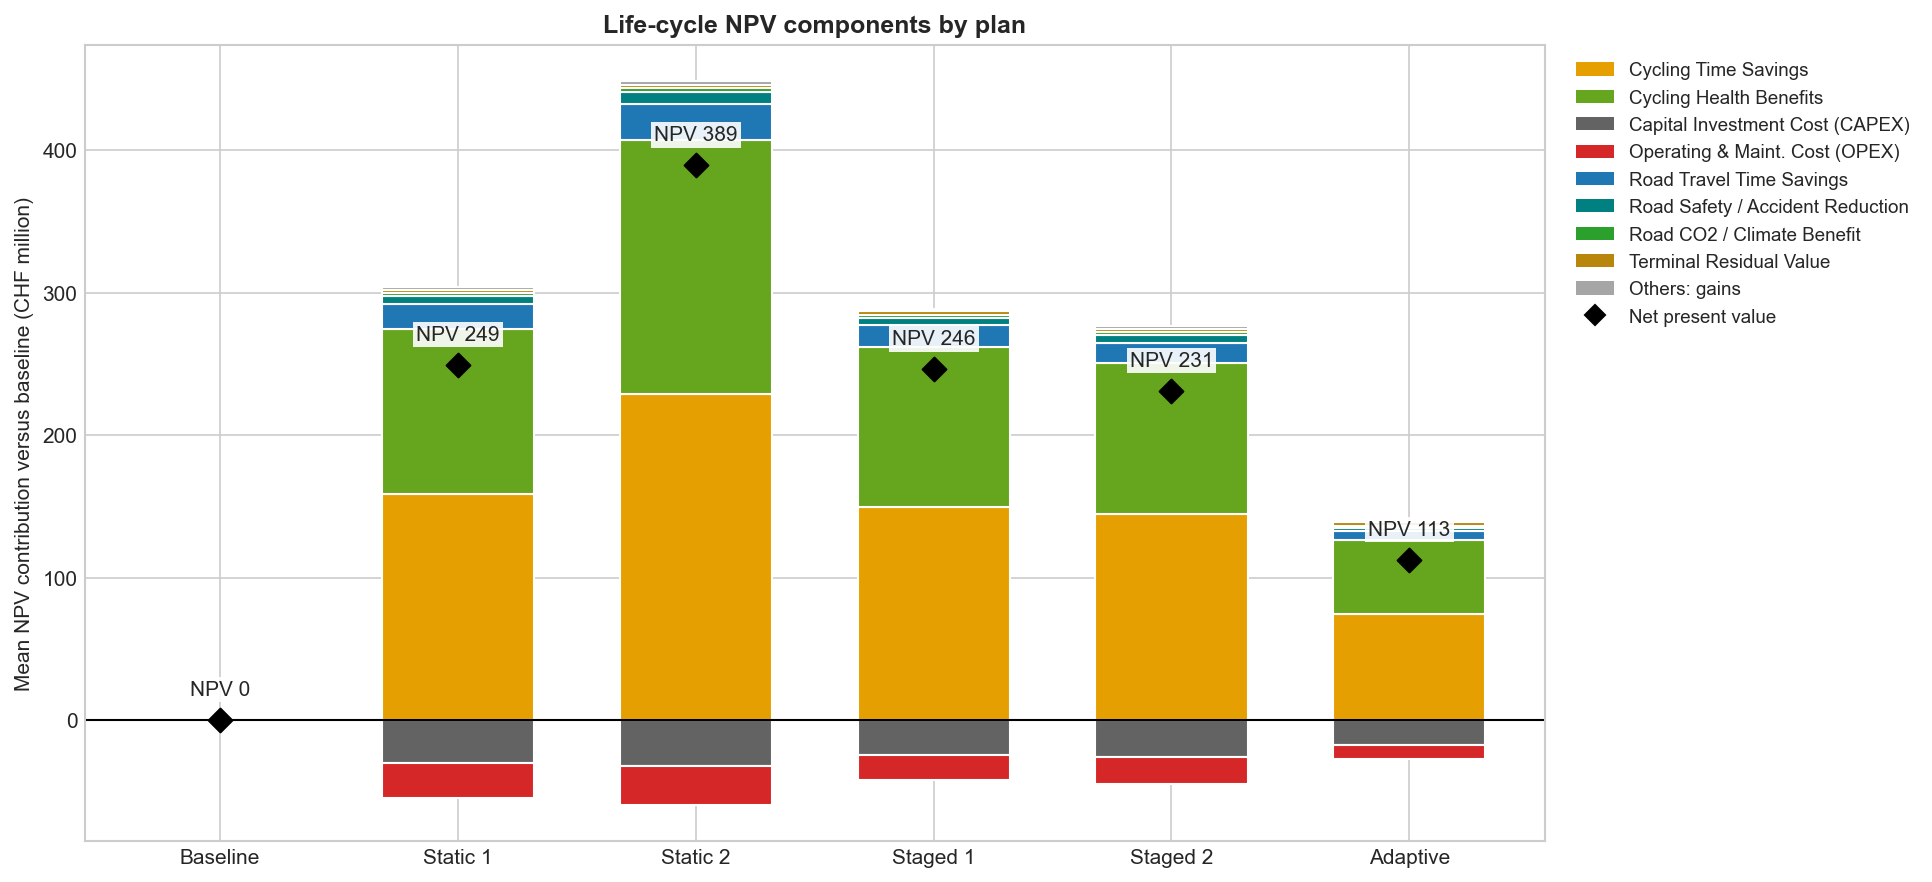
\includegraphics[width=\textwidth]{figures/scenario_ctt_bike_18_7/05_appraisal/05_npv_component_decomposition_mean.png}
\caption{NB05 \S2.2 component breakdown at C\_TT\_BIKE = 18.7: the cycling-time bar shrinks from 428.6 to 229.0\,MCHF (static2); health (177.8) now rivals it.}
\end{figure}

\subsection{NB04 \S1.4 derivative: full adaptive range + paired Year-20/Y40 (added 2026-11-21)}
A new cell after Task 1.4 plots the fixed plans solid and \emph{every one of the 200 adaptive
scenarios} as a hairline (\texttt{alpha=.09, lw=.8}, the run-level styling of the
central-performance plots), so the range of real trigger outcomes is visible instead of the
illustrative dashed placeholders. The paired-transport-change plot (\S3.3) is now emitted for
both Year 40 and Year 20: at Year 40 the staged plans end at "Both stages" and their ECDFs
coincide with static2 (staged1/staged2 purple/red are overdrawn by green), while at Year 20
staged2 (tunnel opens Y25) is still at Stage 1 and visibly distinct. The Year-20 frame is the
one that separates the plans.

\begin{figure}[p]\centering
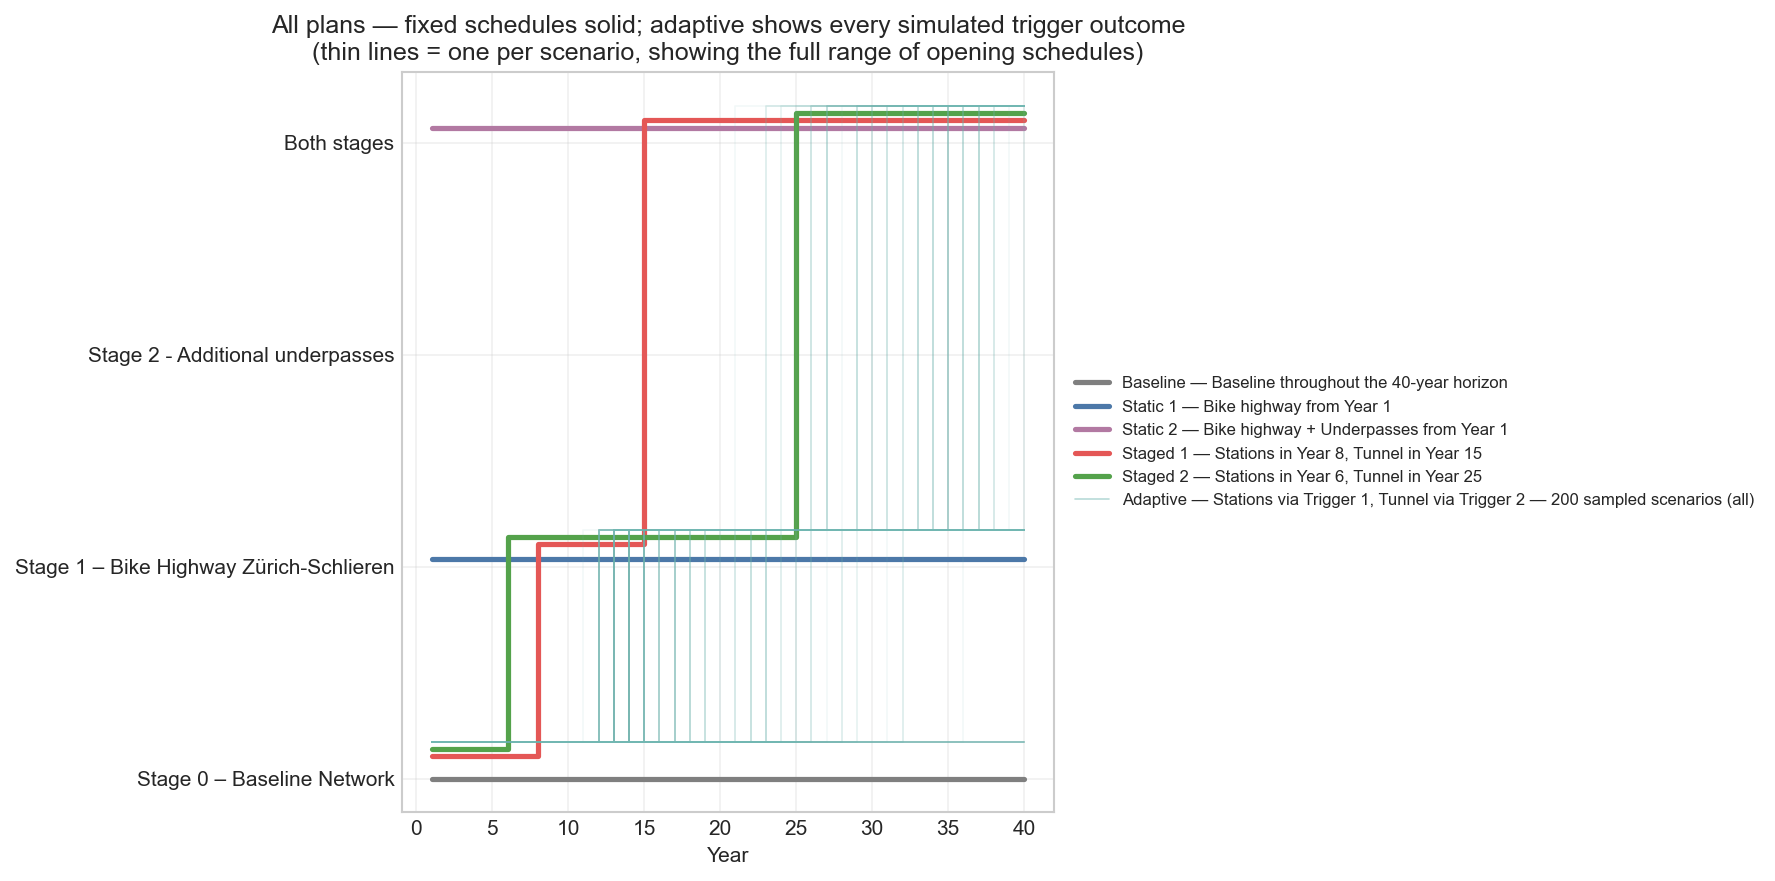
\includegraphics[width=\textwidth]{figures/scenario_ctt_bike_18_7/04_adaptive_planning/04_all_plan_schedules_range.png}
\caption{NB04 \S1.4b: fixed plans solid; all 200 adaptive scenarios as thin teal lines --- the full simulated opening-schedule range.}
\end{figure}
\begin{figure}[p]\centering
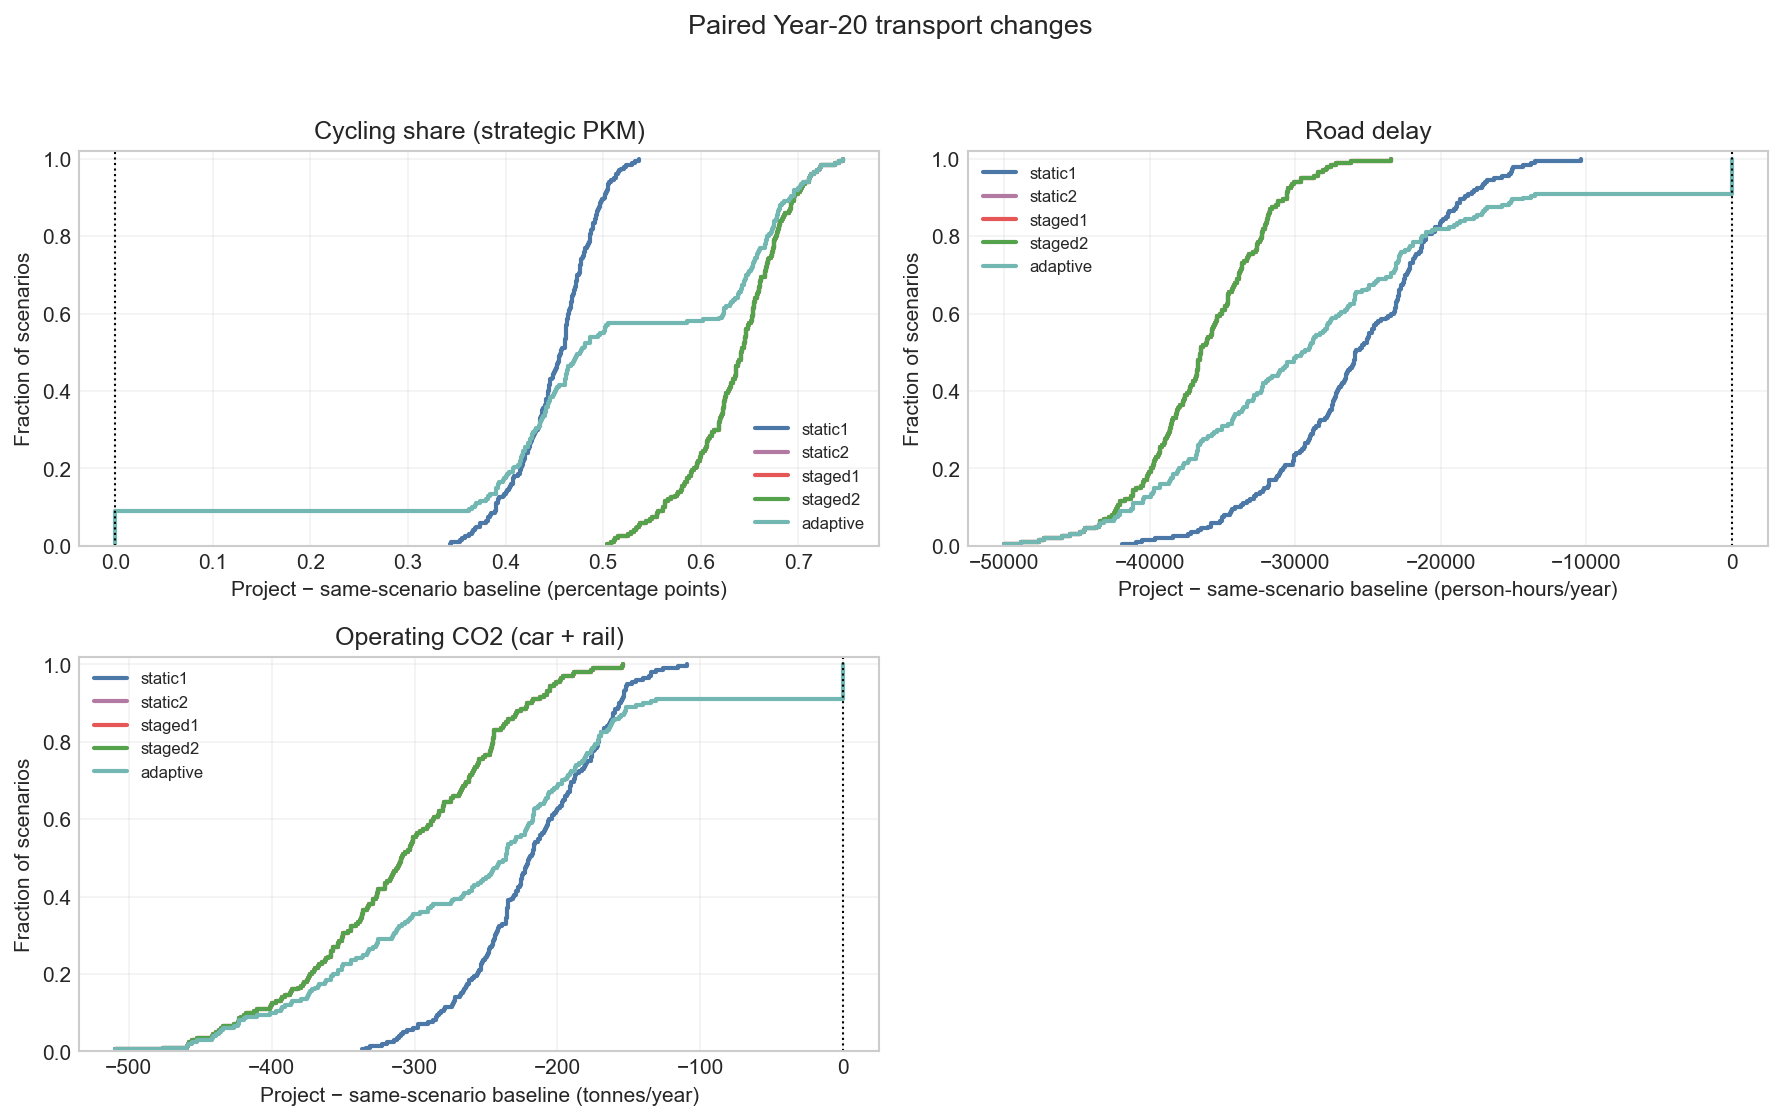
\includegraphics[width=\textwidth]{figures/scenario_ctt_bike_18_7/04_adaptive_planning/03_3_paired_year20.png}
\caption{NB04 \S3.3 at Year 20: staged2 (green) still distinct from static2 before its tunnel opens at Y25; adaptive shows its 9\% zero-delta mass at left.}
\end{figure}

\section{What the figures show (visual read of the fresh NB04/NB05 outputs)}
\subsection{Notebook 04}
\begin{itemize}
\item \textbf{04\_robustness\_requirements.png / 04\_requirement\_robustness.png} --- per-requirement breach bars: req3 fails in 97--99\% of scenarios for every plan; req1 in $\approx$78--90\% (build plans lower than baseline/adaptive); req2 in $\approx$27--46\%. The ``all requirements all years'' panel shows only $\approx$1.5--3\% bars for every plan, with mean failure duration $\approx$15--16 years (p90 = 21, the full window).
\item \textbf{04\_2\_requirement\_failures.png} --- failure curves are flat at 0\% until the dashed Year-20 line, then jump (req3 to $\approx$97\%, req1 to $\approx$85--90\%, req2 to $\approx$30--45\%) and decay gradually to Year 40; build stages consistently sit below baseline. First failures are exactly Year 20 everywhere.
\item \textbf{04\_fan\_Baseline\_static.png / 04\_fan\_Staged.png / 04\_fan\_Adaptive.png} --- median Year-40 bike share $\approx$12.6--13.5\% for build plans vs $\approx$12.6\% adaptive (crossing the 12\% line only $\approx$Year 29--33, staged2 earliest $\approx$Year 26); all uncertainty bands overlap heavily, so higher medians do not imply robustness.
\item \textbf{04\_adaptive\_trigger\_buckets.png / 05\_5\_pathway\_frequencies.png / 05\_1\_opening\_distributions.png} --- in the base run (old 44k/60k triggers) the monitored indicator never approached the trigger lines (pathway chart: ``no package open'' = 100\%); in \texttt{figures/scenario\_triggers/} with the recalibrated +20\%/+50\% triggers the same panels show Stage 1 opening in 73.5\% and Stage 2 in 42.5\% of scenarios.
\item \textbf{04\_parcoords\_plan\_summary.png} --- static2 leads on physical axes, adaptive sits at 0 on all physical axes and $\approx$1 on cost: the value-vs-money trade-off in one plot.
\item \textbf{04\_prim\_comparison.png} --- vulnerability boxes in BIKE\_ASC\_SHIFT $\times$ EBIKE\_SHARE space: req-2 failure boundary at BIKE\_ASC\_SHIFT $\approx$0.33, req-1 at $\approx$0.53 (the numbers confirm: failures are the \emph{low}-preference side; the subagent's plot read had the box mirrored); baseline and adaptive columns identical.
\item \textbf{04\_4\_restoration\_windows.png} --- restoration windows exist only in Years $\approx$20--40, and some scenario/package combos have none at all: reacting after failures start (Year 20) with 10-year lead times leaves little horizon to recover.
\item \textbf{03\_3\_paired\_year40.png} --- paired Year-40 deltas are one-sided and tight: every build plan improves bike share (+0.33 to +0.74 pp), road delay ($-$10k to $-$50k person-h/yr) and CO2 ($-$110 to $-$500 t/yr) in every scenario; baseline/adaptive collapse at 0.
\item \textbf{05\_6\_value\_and\_price\_of\_waiting.png} --- 96\% of scenarios: 0 extra failure years for waiting; expenditure saving $\approx$9--53\,MCHF (mean $\approx$28--30\,MCHF); 4\% buy exactly 1 extra failure year for more saving.
\end{itemize}

\subsection{Notebook 05}
\begin{itemize}
\item \textbf{05\_npv\_performance.png} --- ECDFs: all build plans 100\% above zero (static2 up to $\approx$1{,}100\,MCHF), adaptive a vertical line at $\approx-$2\,MCHF.
\item \textbf{05\_joint\_value\_and\_requirement\_outcomes.png / 05\_vulnerability\_by\_plan.png} --- no plan reaches the top-right ``value \emph{and} robust'' corner; builds are 97\% ``NPV only'', adaptive is 100\% negative-NPV and fails requirements exactly like baseline (90.5/46.5/98.5\%).
\item \textbf{05\_downside\_and\_regret.png} --- worst-10\% NPV still positive for builds (static2 +731\,MCHF), regret: static2 = 0, staged $\approx$210--220, static1 $\approx$284--328, adaptive $\approx$860\,MCHF (the whole value gap).
\item \textbf{05\_waiting\_value\_protection\_tradeoffs.png / 05\_waiting\_component\_differences.png} --- waiting saves $\approx$32--61\,MCHF expenditure but loses $-$500 to $-$1{,}050\,MCHF of value: the price of waiting is $\approx$10--20$\times$ the saving; component waterfall shows the entire saving is CAPEX/OPEX, overwhelmed by lost time-and-access benefits.
\item \textbf{05\_threshold\_optimization\_heatmap.png} --- NPV surface over trigger-1 $\times$ trigger-2 thresholds is flat at $\approx-$2\,MCHF everywhere (no trigger ever fires), so threshold tuning cannot rescue the adaptive plan; the ``best tested'' star is noise on a flat plane.
\item \textbf{05\_appraisal\_sensitivity\_tornado.png / 05\_npv\_component\_decomposition\_mean.png / 05\_component\_nvp\_ecdf\_grid.png} --- appraisal conclusions are stable to assumption swings; value is cycling time + health; only build plans realize it.
\item \textbf{05\_prim\_box\_overlay.png} --- in demand $\times$ PT-preference space the failure regions are diffuse; the discriminating axis is BIKE\_ASC\_SHIFT (see NB04 PRIM).
\end{itemize}

\subsection{Figures}
\begin{figure}[p]\centering
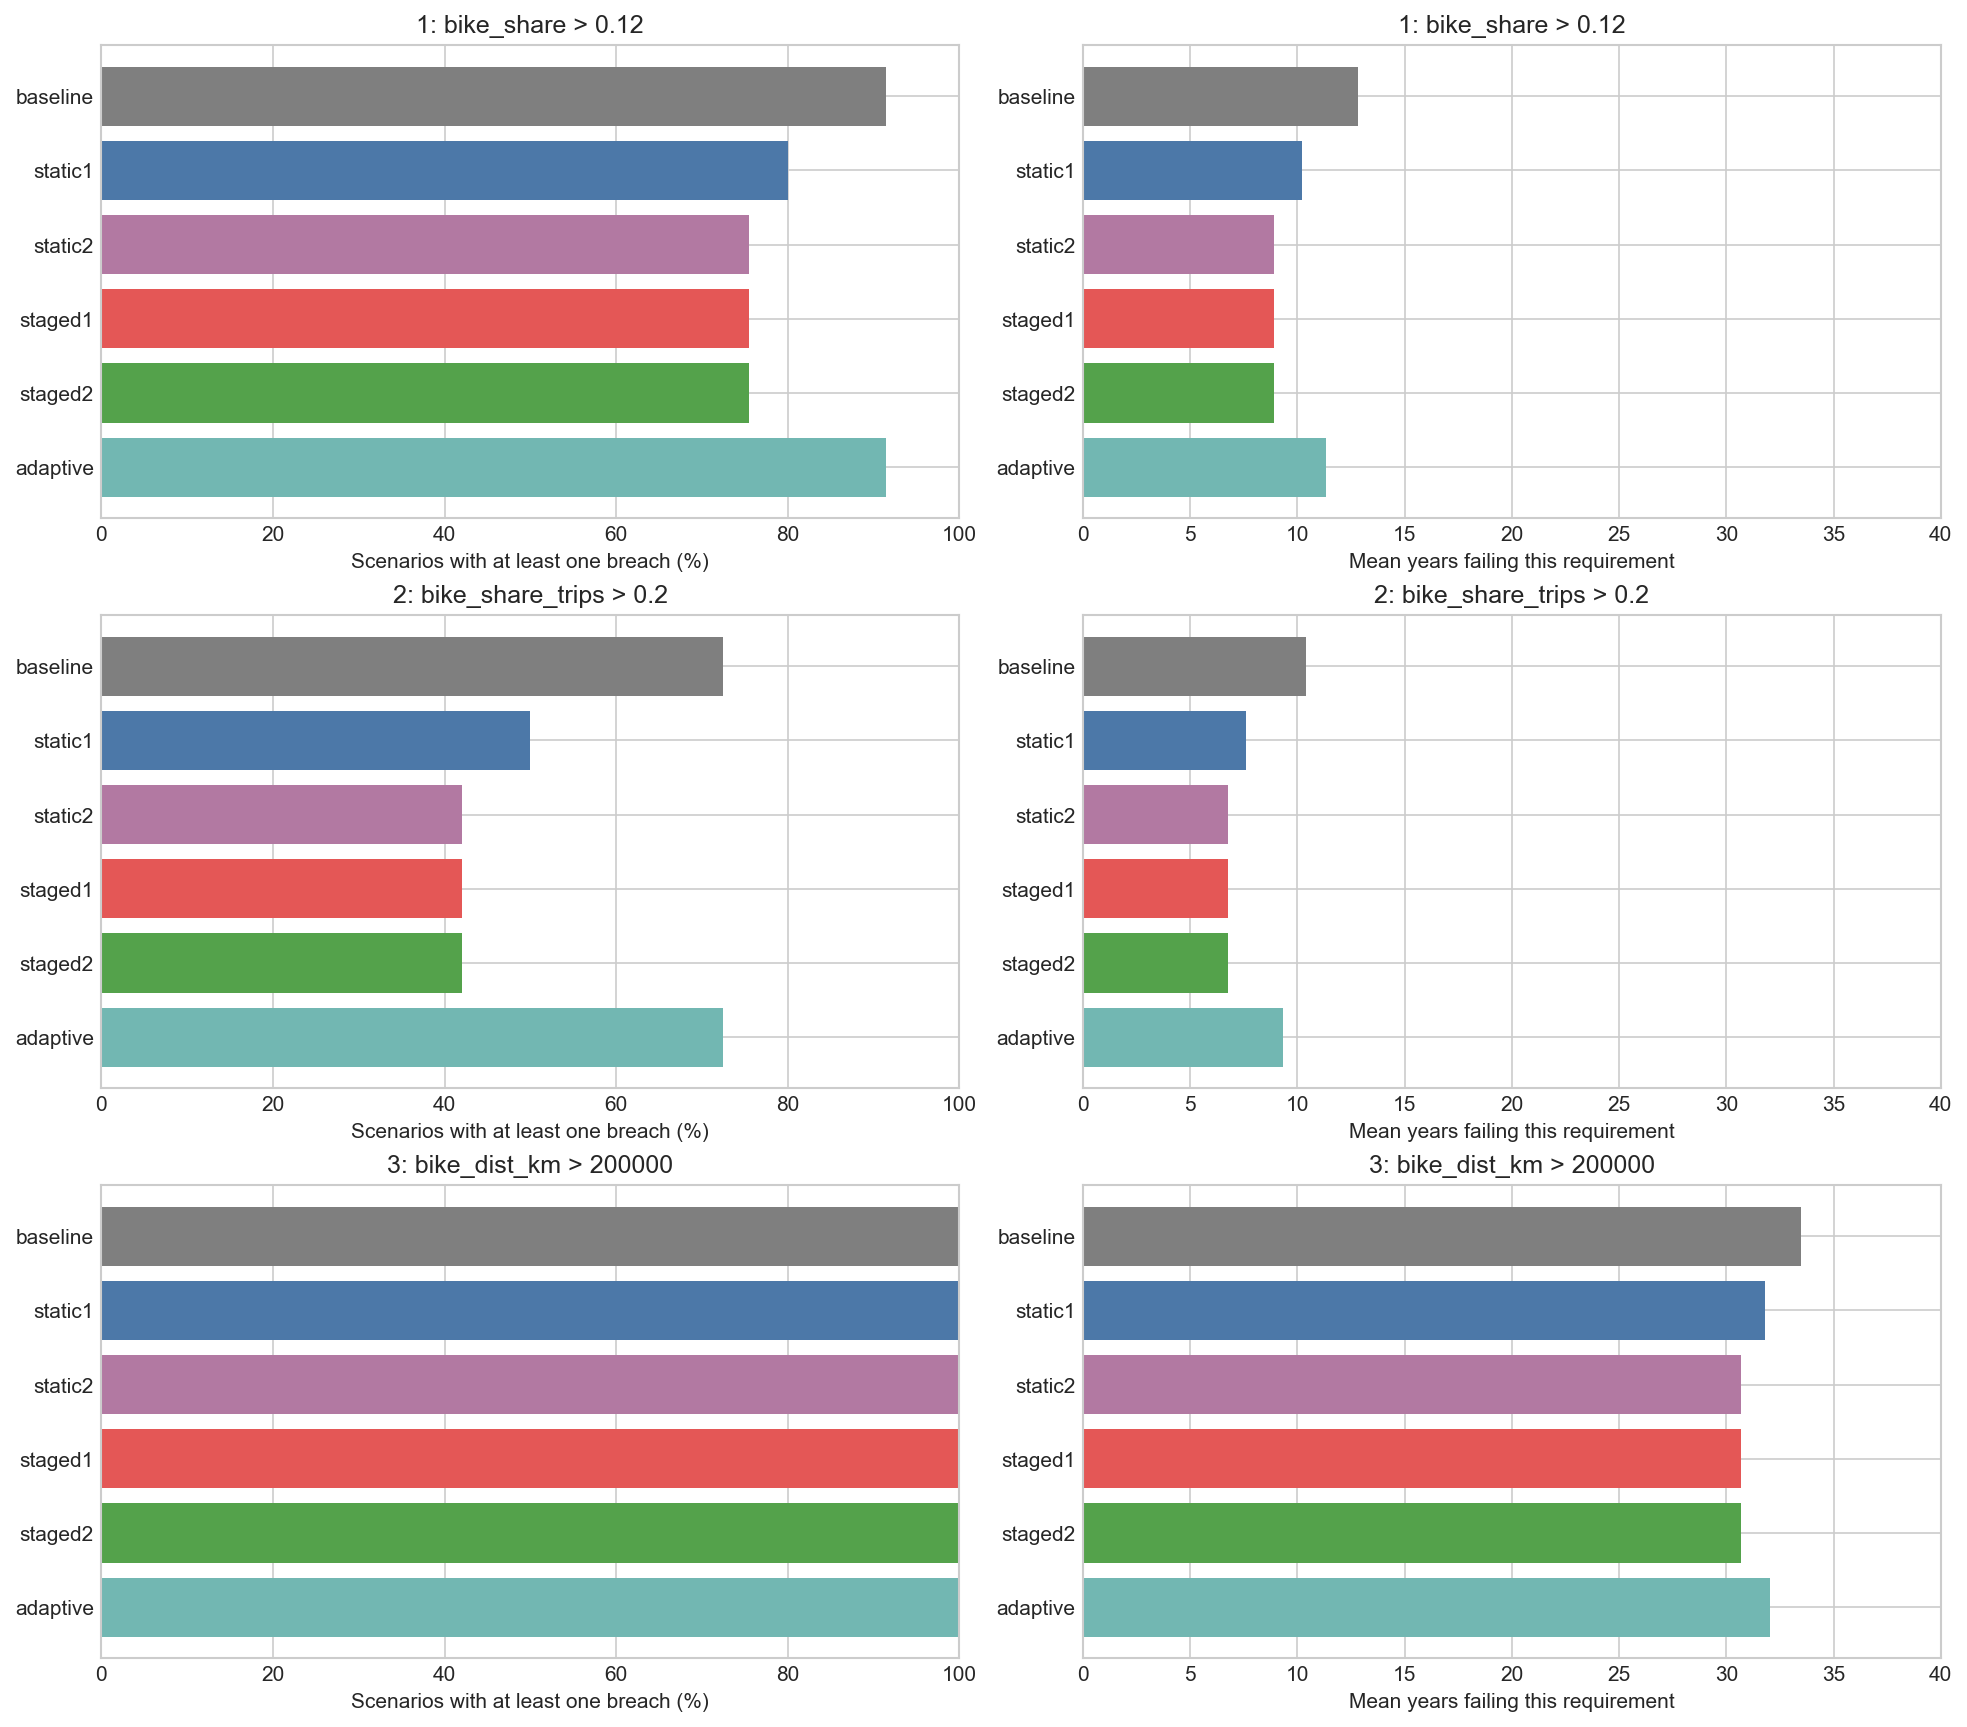
\includegraphics[width=\textwidth]{figures/04_adaptive_planning/04_requirement_robustness.png}
\caption{NB04: per-requirement robustness (breach share and failure duration by plan).}
\end{figure}
\begin{figure}[p]\centering
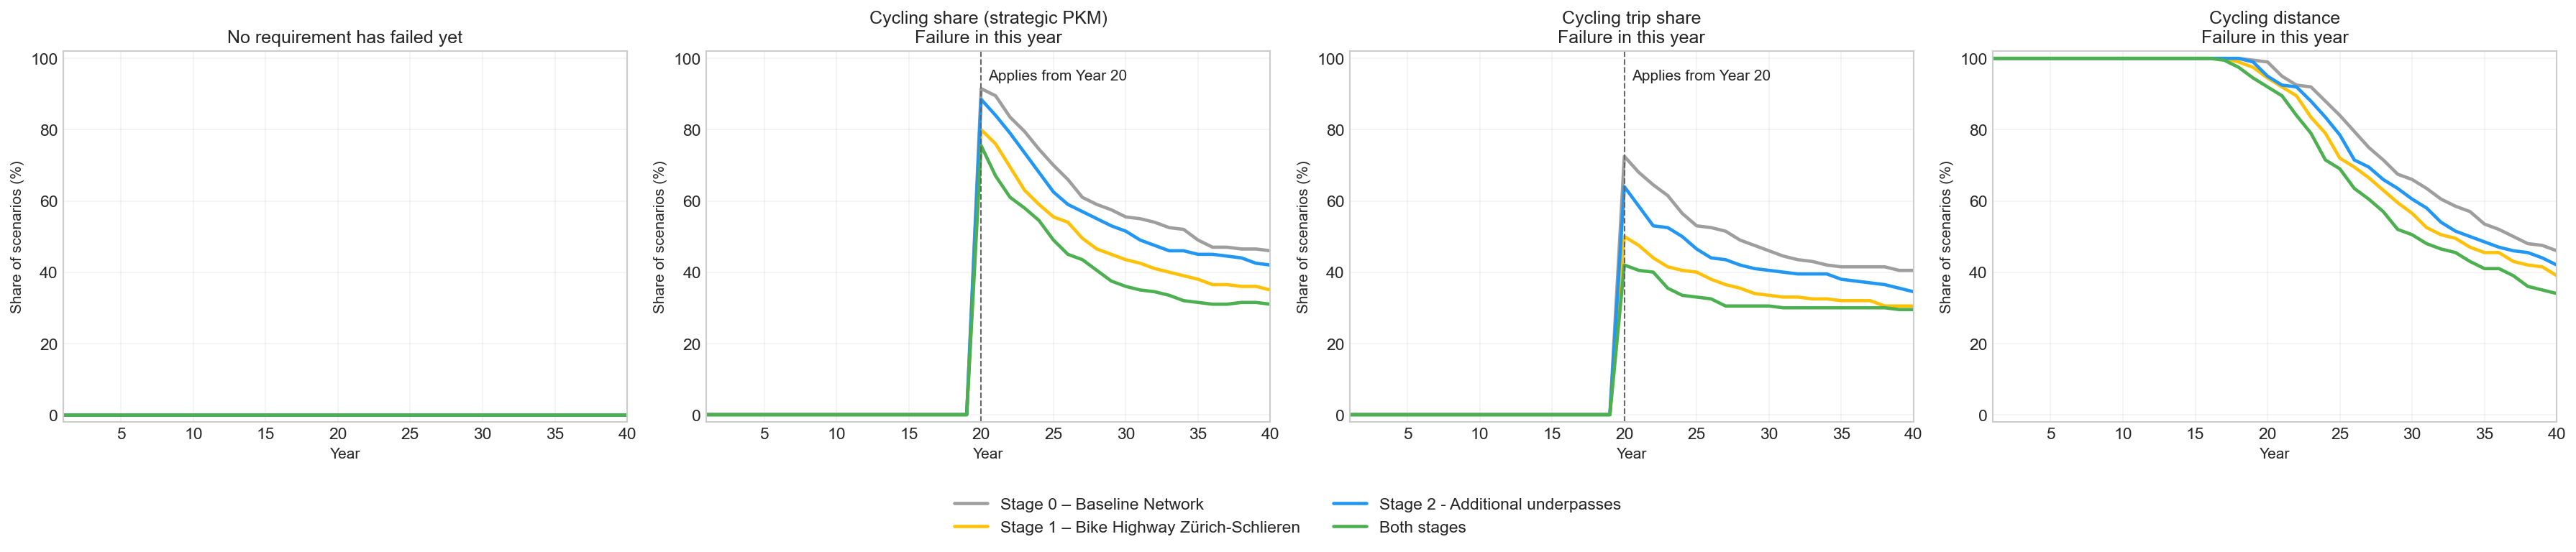
\includegraphics[width=\textwidth]{figures/04_adaptive_planning/04_2_requirement_failures.png}
\caption{NB04: failure share by year; all curves jump exactly at the Year-20 requirement start.}
\end{figure}
\begin{figure}[p]\centering
\includegraphics[width=\textwidth]{figures/04_adaptive_planning/05_5_pathway_frequencies.png}
\caption{NB04: adaptive pathway frequencies --- ``no package open'' in 100\% of scenarios.}
\end{figure}
\begin{figure}[p]\centering
\includegraphics[width=\textwidth]{figures/04_adaptive_planning/04_adaptive_trigger_buckets.png}
\caption{NB04: monitored bike\_trips median vs. the 44k/60k trigger lines --- never approached.}
\end{figure}
\begin{figure}[p]\centering
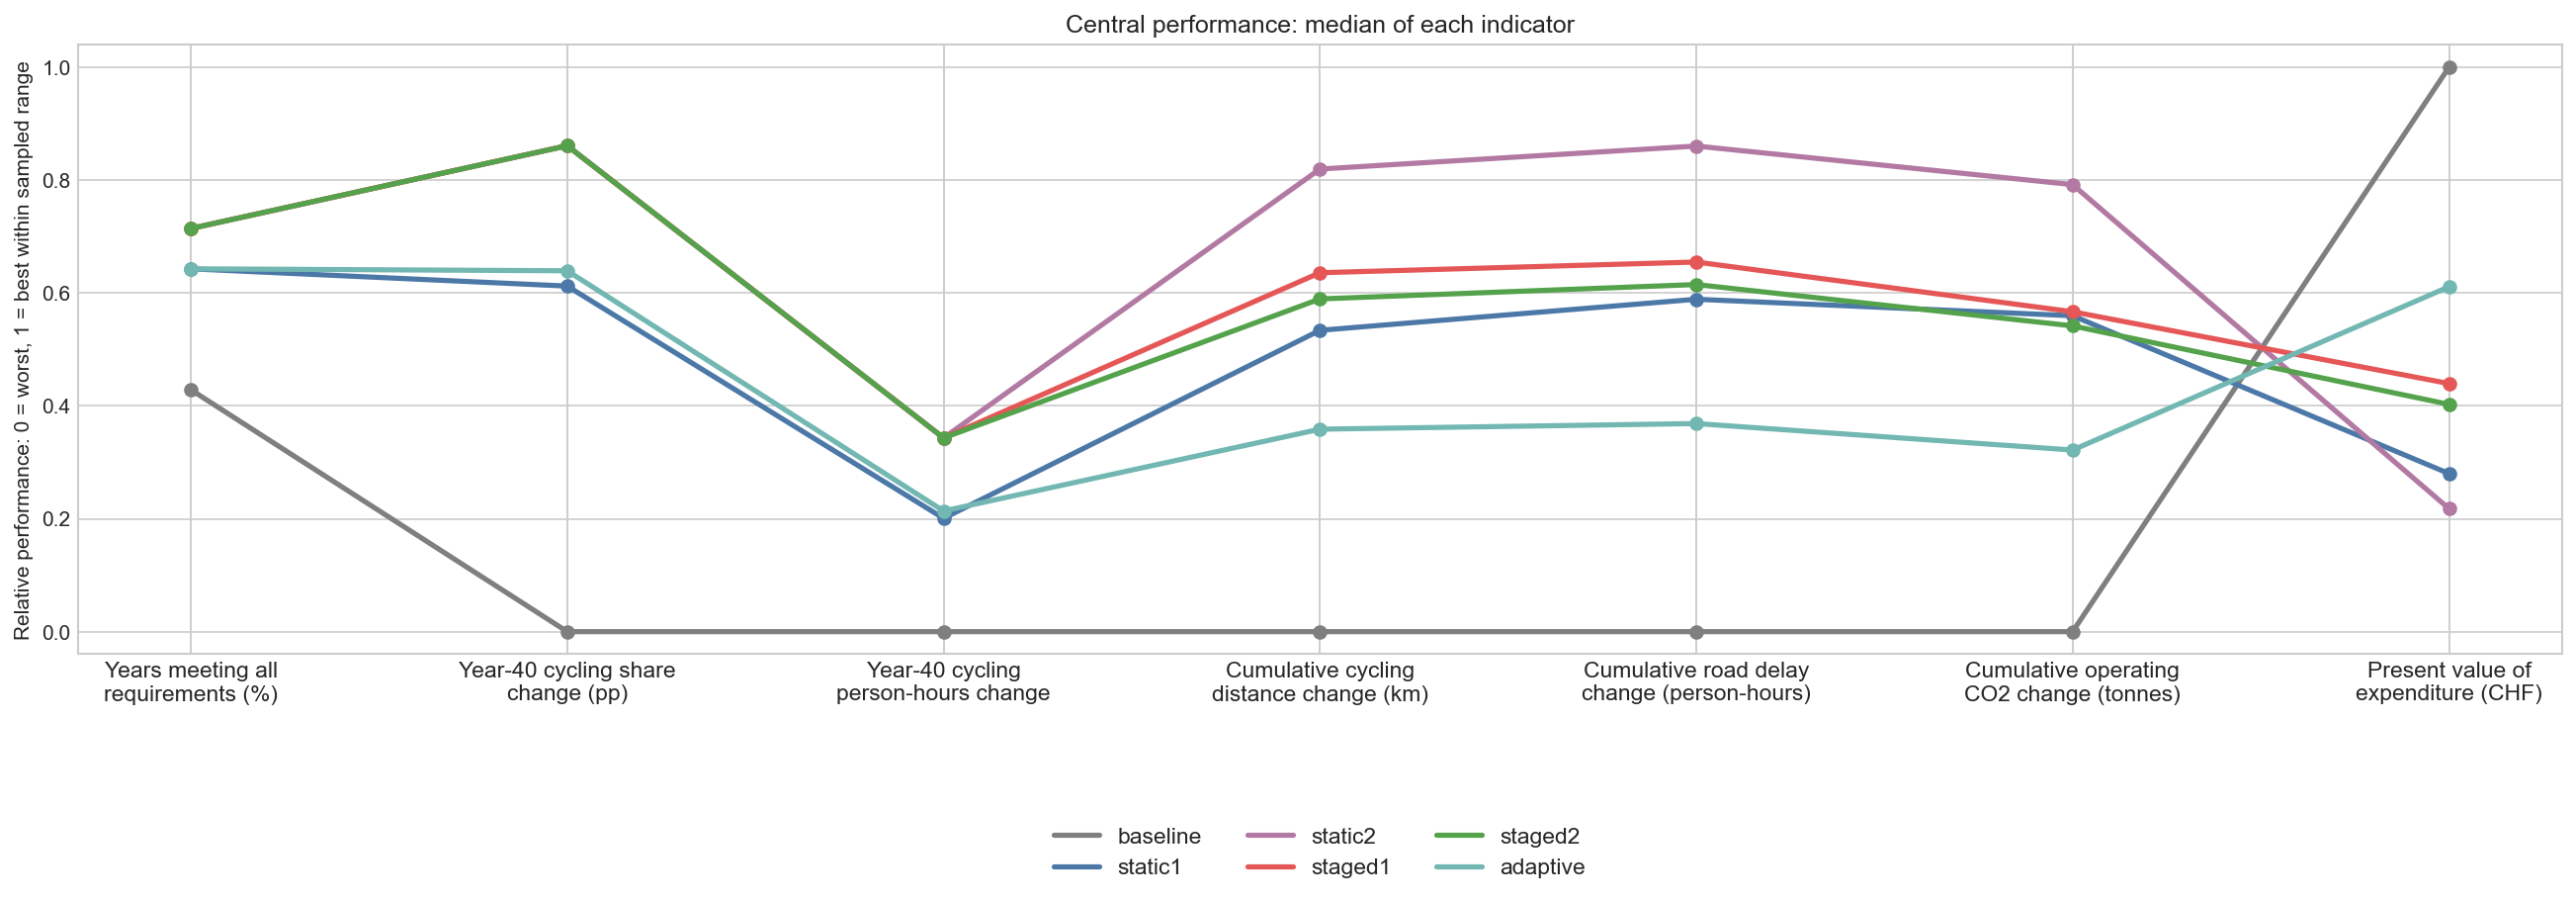
\includegraphics[width=\textwidth]{figures/04_adaptive_planning/04_parcoords_plan_summary.png}
\caption{NB04: plan medians across all axes --- cost vs. physical performance trade-off.}
\end{figure}
\begin{figure}[p]\centering
\includegraphics[width=\textwidth]{figures/05_appraisal/05_npv_performance.png}
\caption{NB05: NPV distributions --- build plans 100\% positive, adaptive at $\approx-$2\,MCHF.}
\end{figure}
\begin{figure}[p]\centering
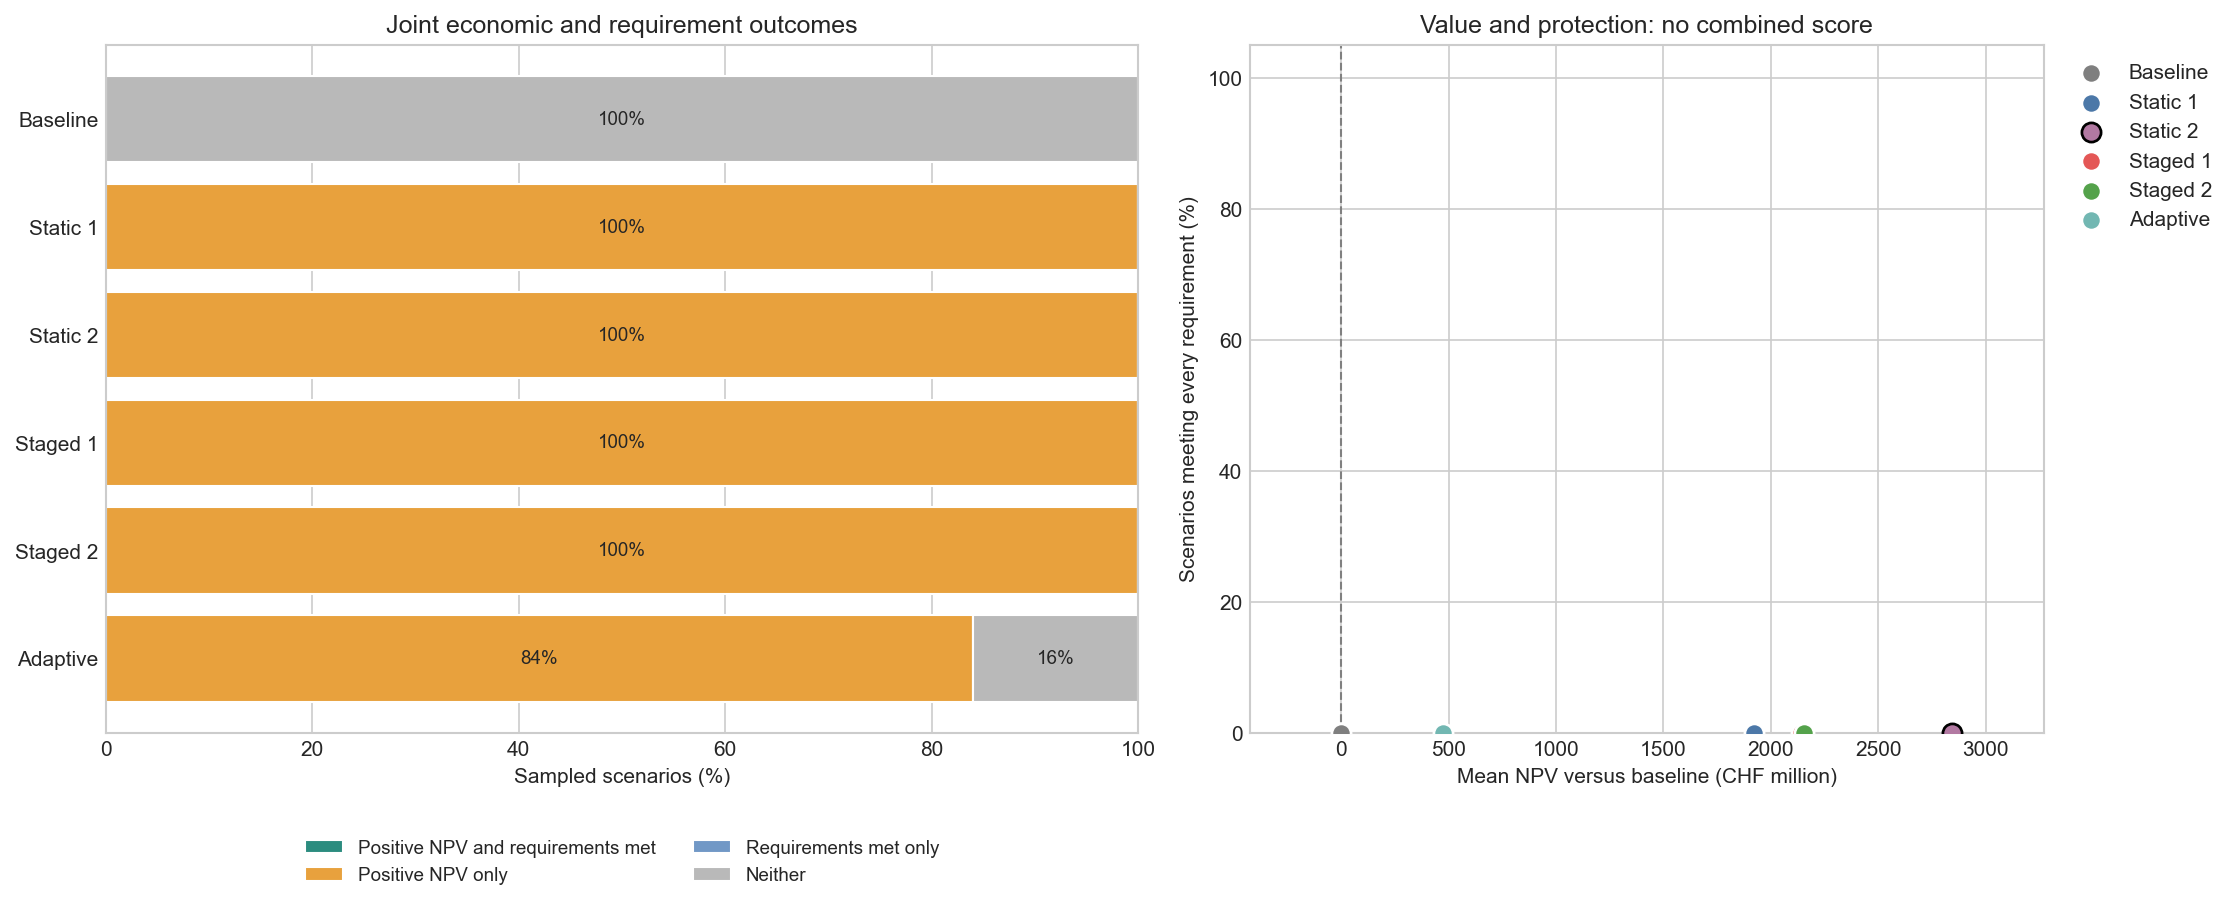
\includegraphics[width=\textwidth]{figures/05_appraisal/05_joint_value_and_requirement_outcomes.png}
\caption{NB05: joint economic-value $\times$ requirement outcomes --- no plan achieves both.}
\end{figure}
\begin{figure}[p]\centering
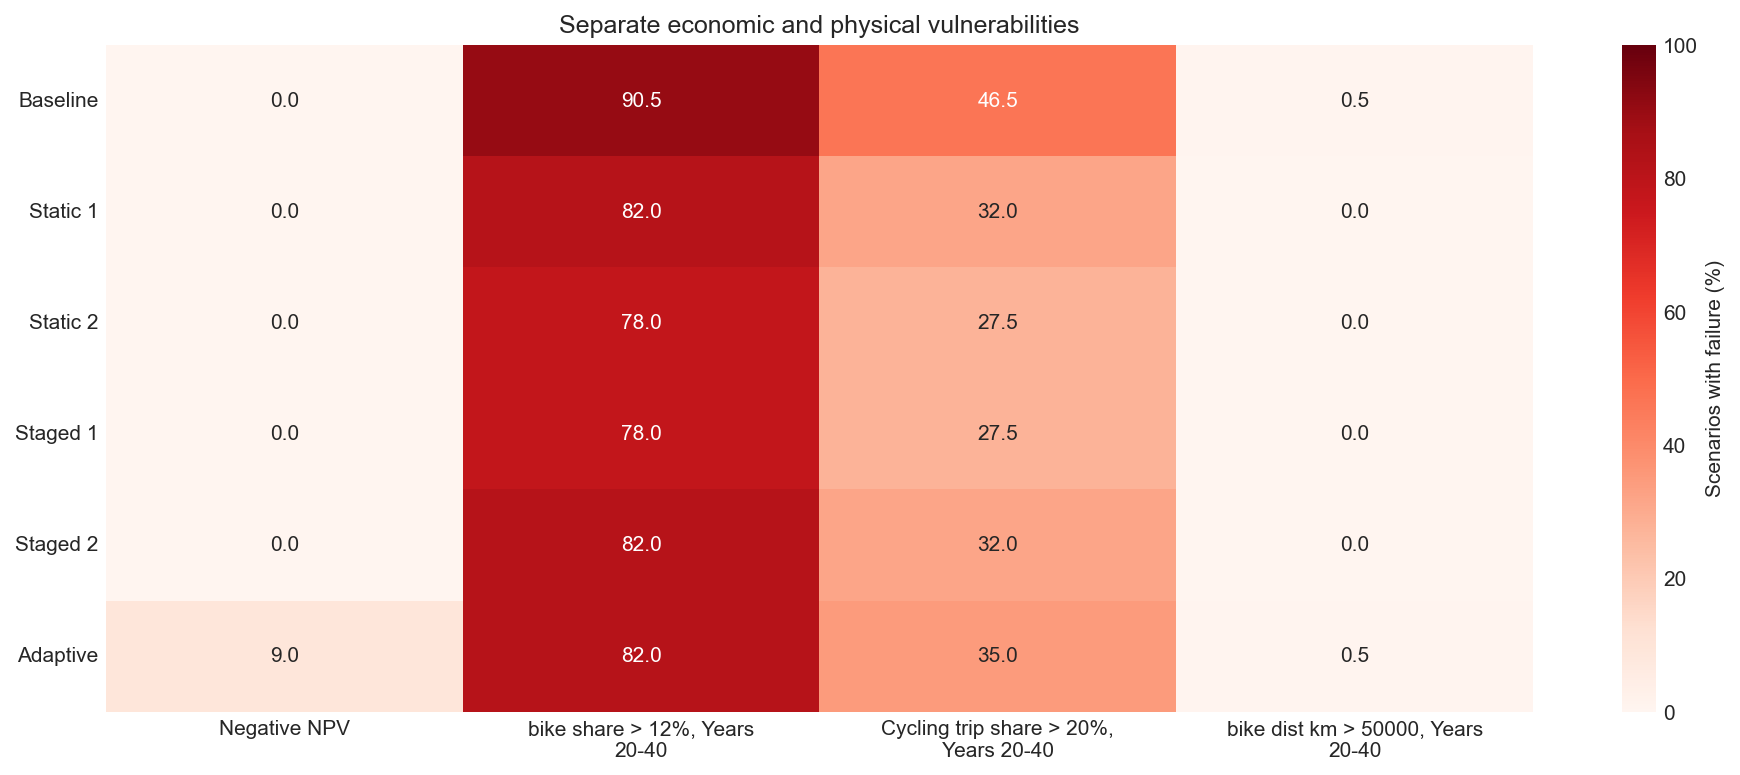
\includegraphics[width=\textwidth]{figures/05_appraisal/05_vulnerability_by_plan.png}
\caption{NB05: vulnerability heatmap --- adaptive fails physically exactly like baseline, and economically in 100\%.}
\end{figure}
\begin{figure}[p]\centering
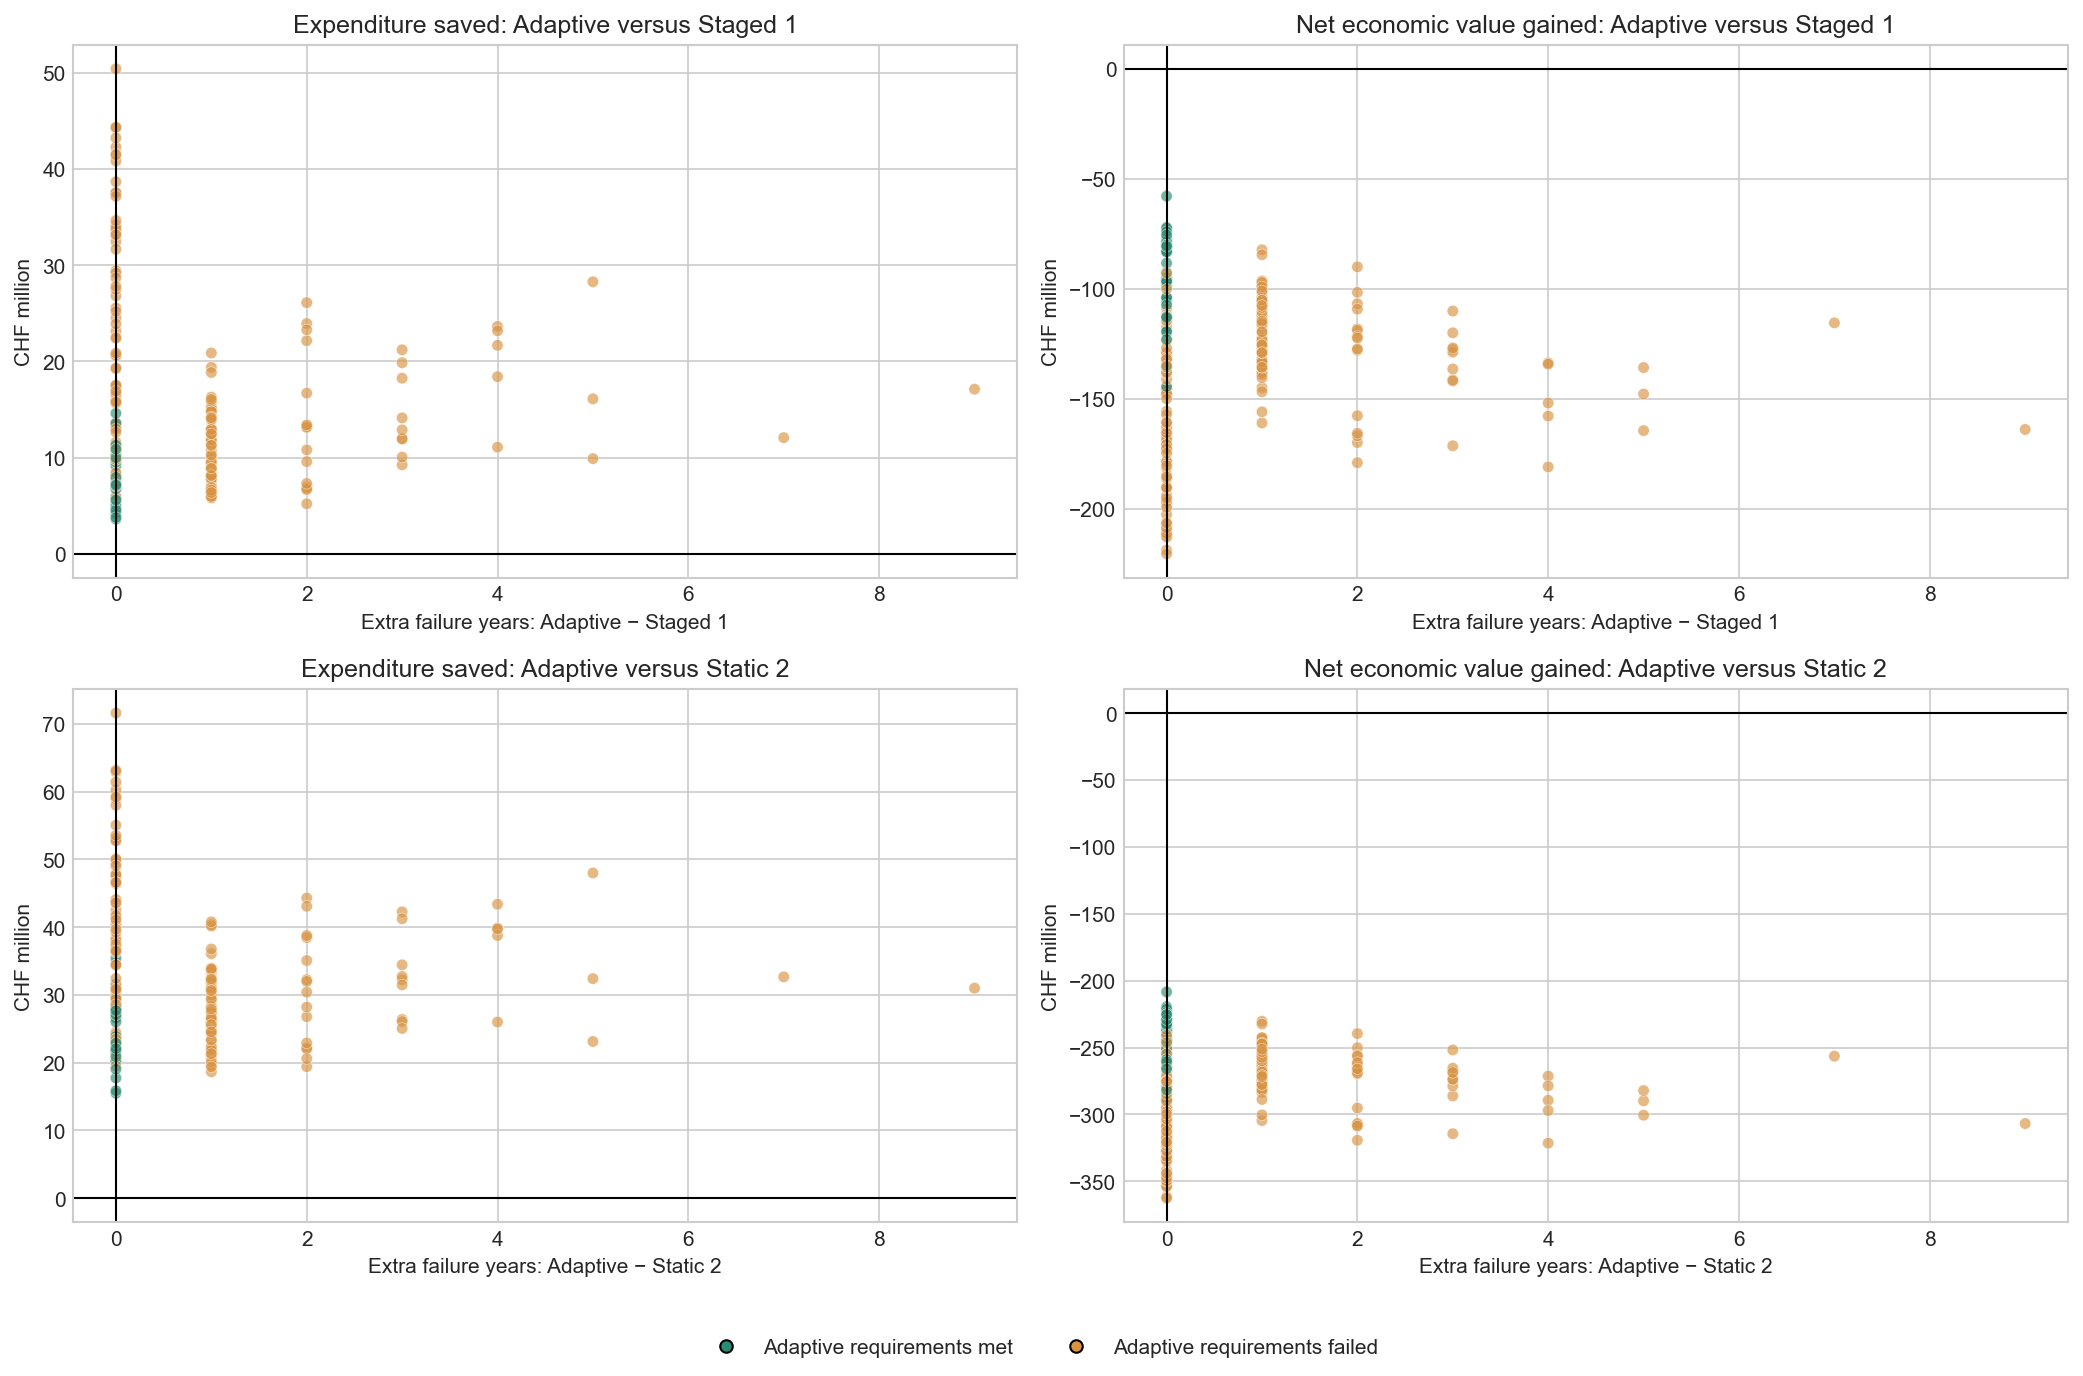
\includegraphics[width=\textwidth]{figures/05_appraisal/05_waiting_value_protection_tradeoffs.png}
\caption{NB05: waiting saves 32--61\,MCHF but forfeits 500--1{,}050\,MCHF of NPV.}
\end{figure}
\begin{figure}[p]\centering
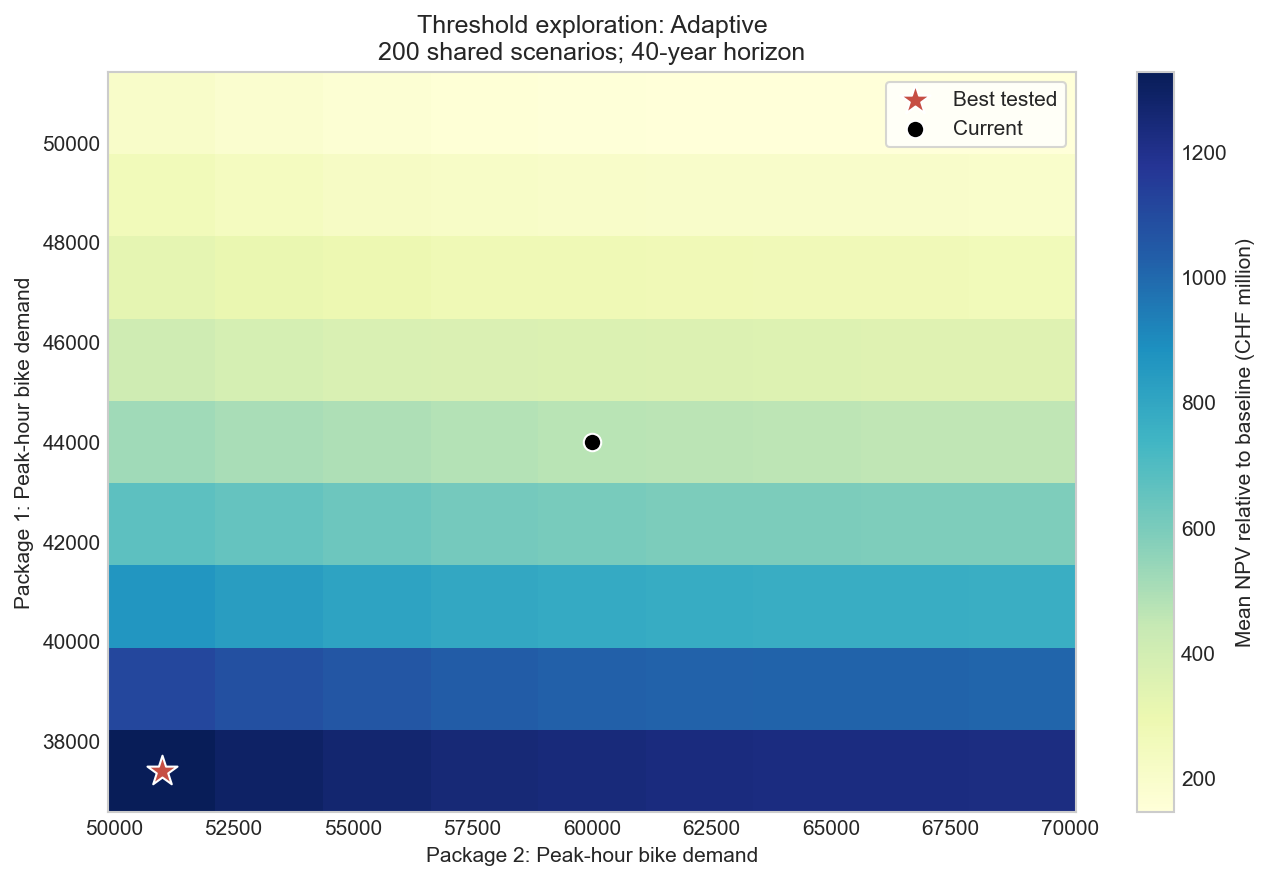
\includegraphics[width=\textwidth]{figures/05_appraisal/05_threshold_optimization_heatmap.png}
\caption{NB05: NPV over trigger thresholds is flat --- no trigger setting rescues the adaptive plan.}
\end{figure}
\begin{figure}[p]\centering
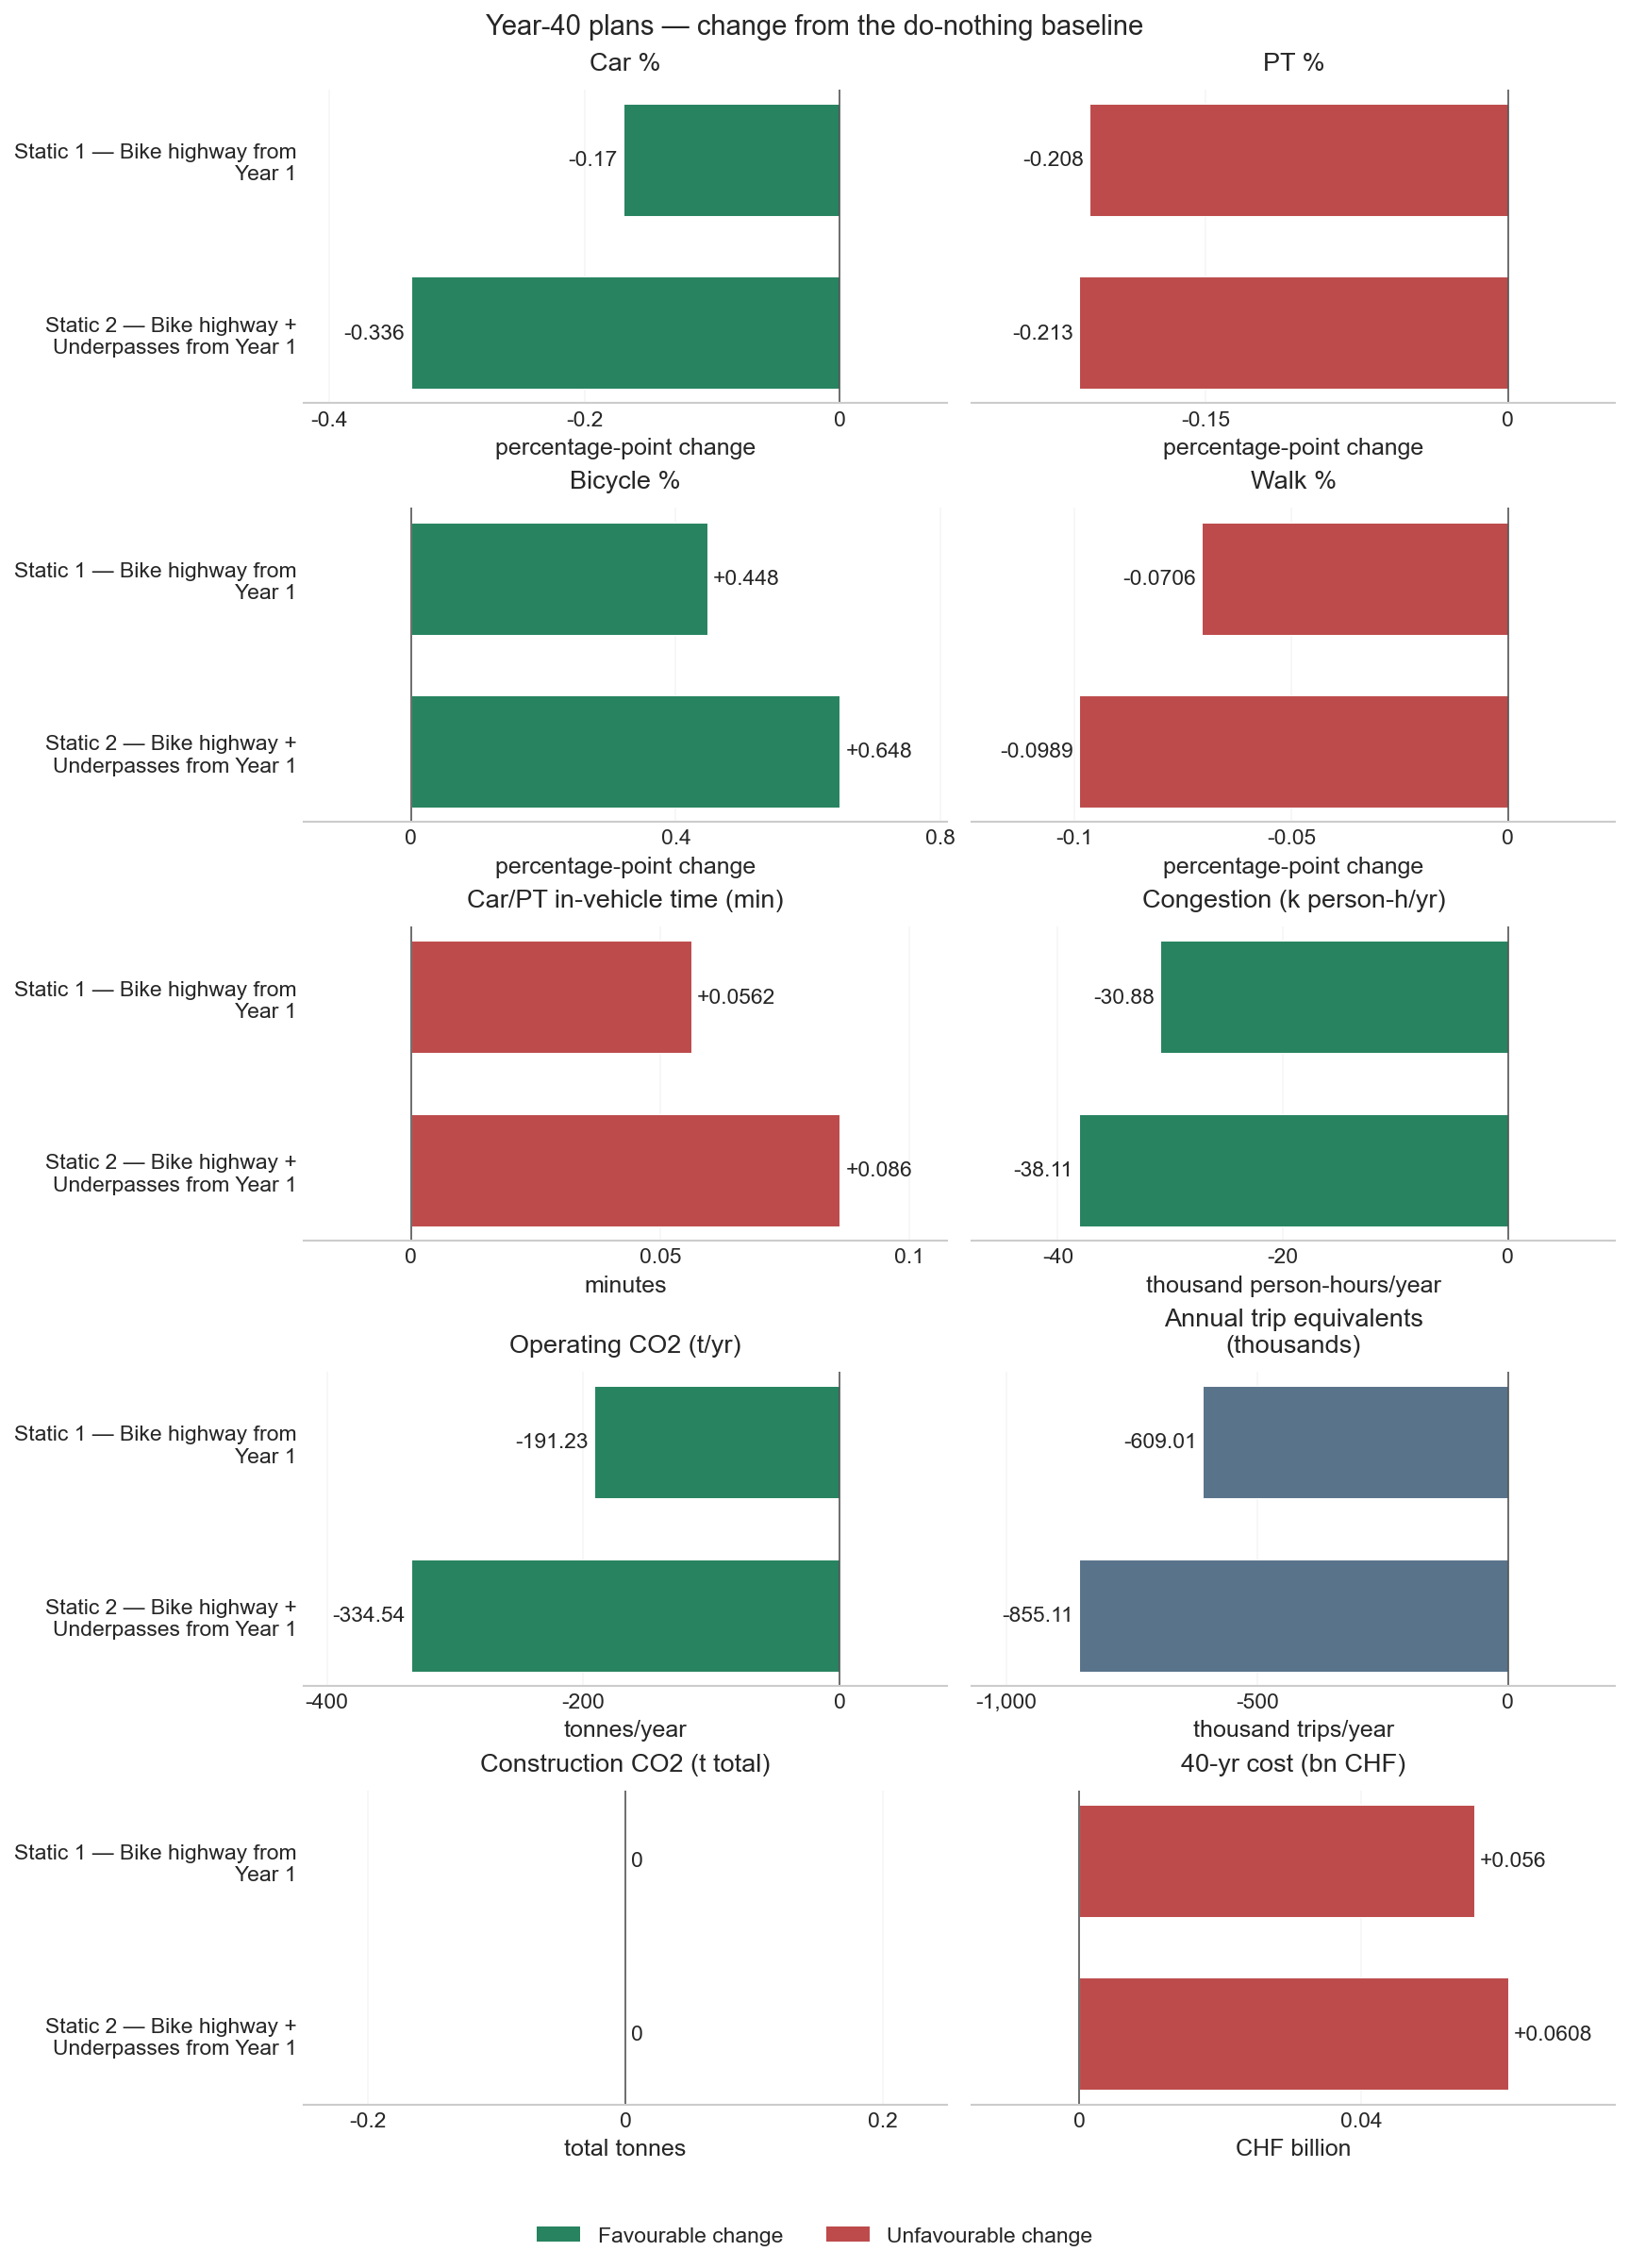
\includegraphics[width=\textwidth]{figures/02_plan_outcomes_changes.png}
\caption{NB02: static-plan Year-40 deltas (bike share +0.45/+0.65 pp, congestion $-$31k/$-$38k h/yr, CO$_2$ $-$191/$-$334 t/yr).}
\end{figure}

\begin{figure}[p]\centering
\includegraphics[width=\textwidth]{figures/scenario_triggers/04_adaptive_planning/05_5_pathway_frequencies.png}
\caption{NB04 with recalibrated triggers (scenario\_triggers): pathway frequencies --- 42.5\% both stages, 31\% Stage 1 only, 26.5\% none.}
\end{figure}
\begin{figure}[p]\centering
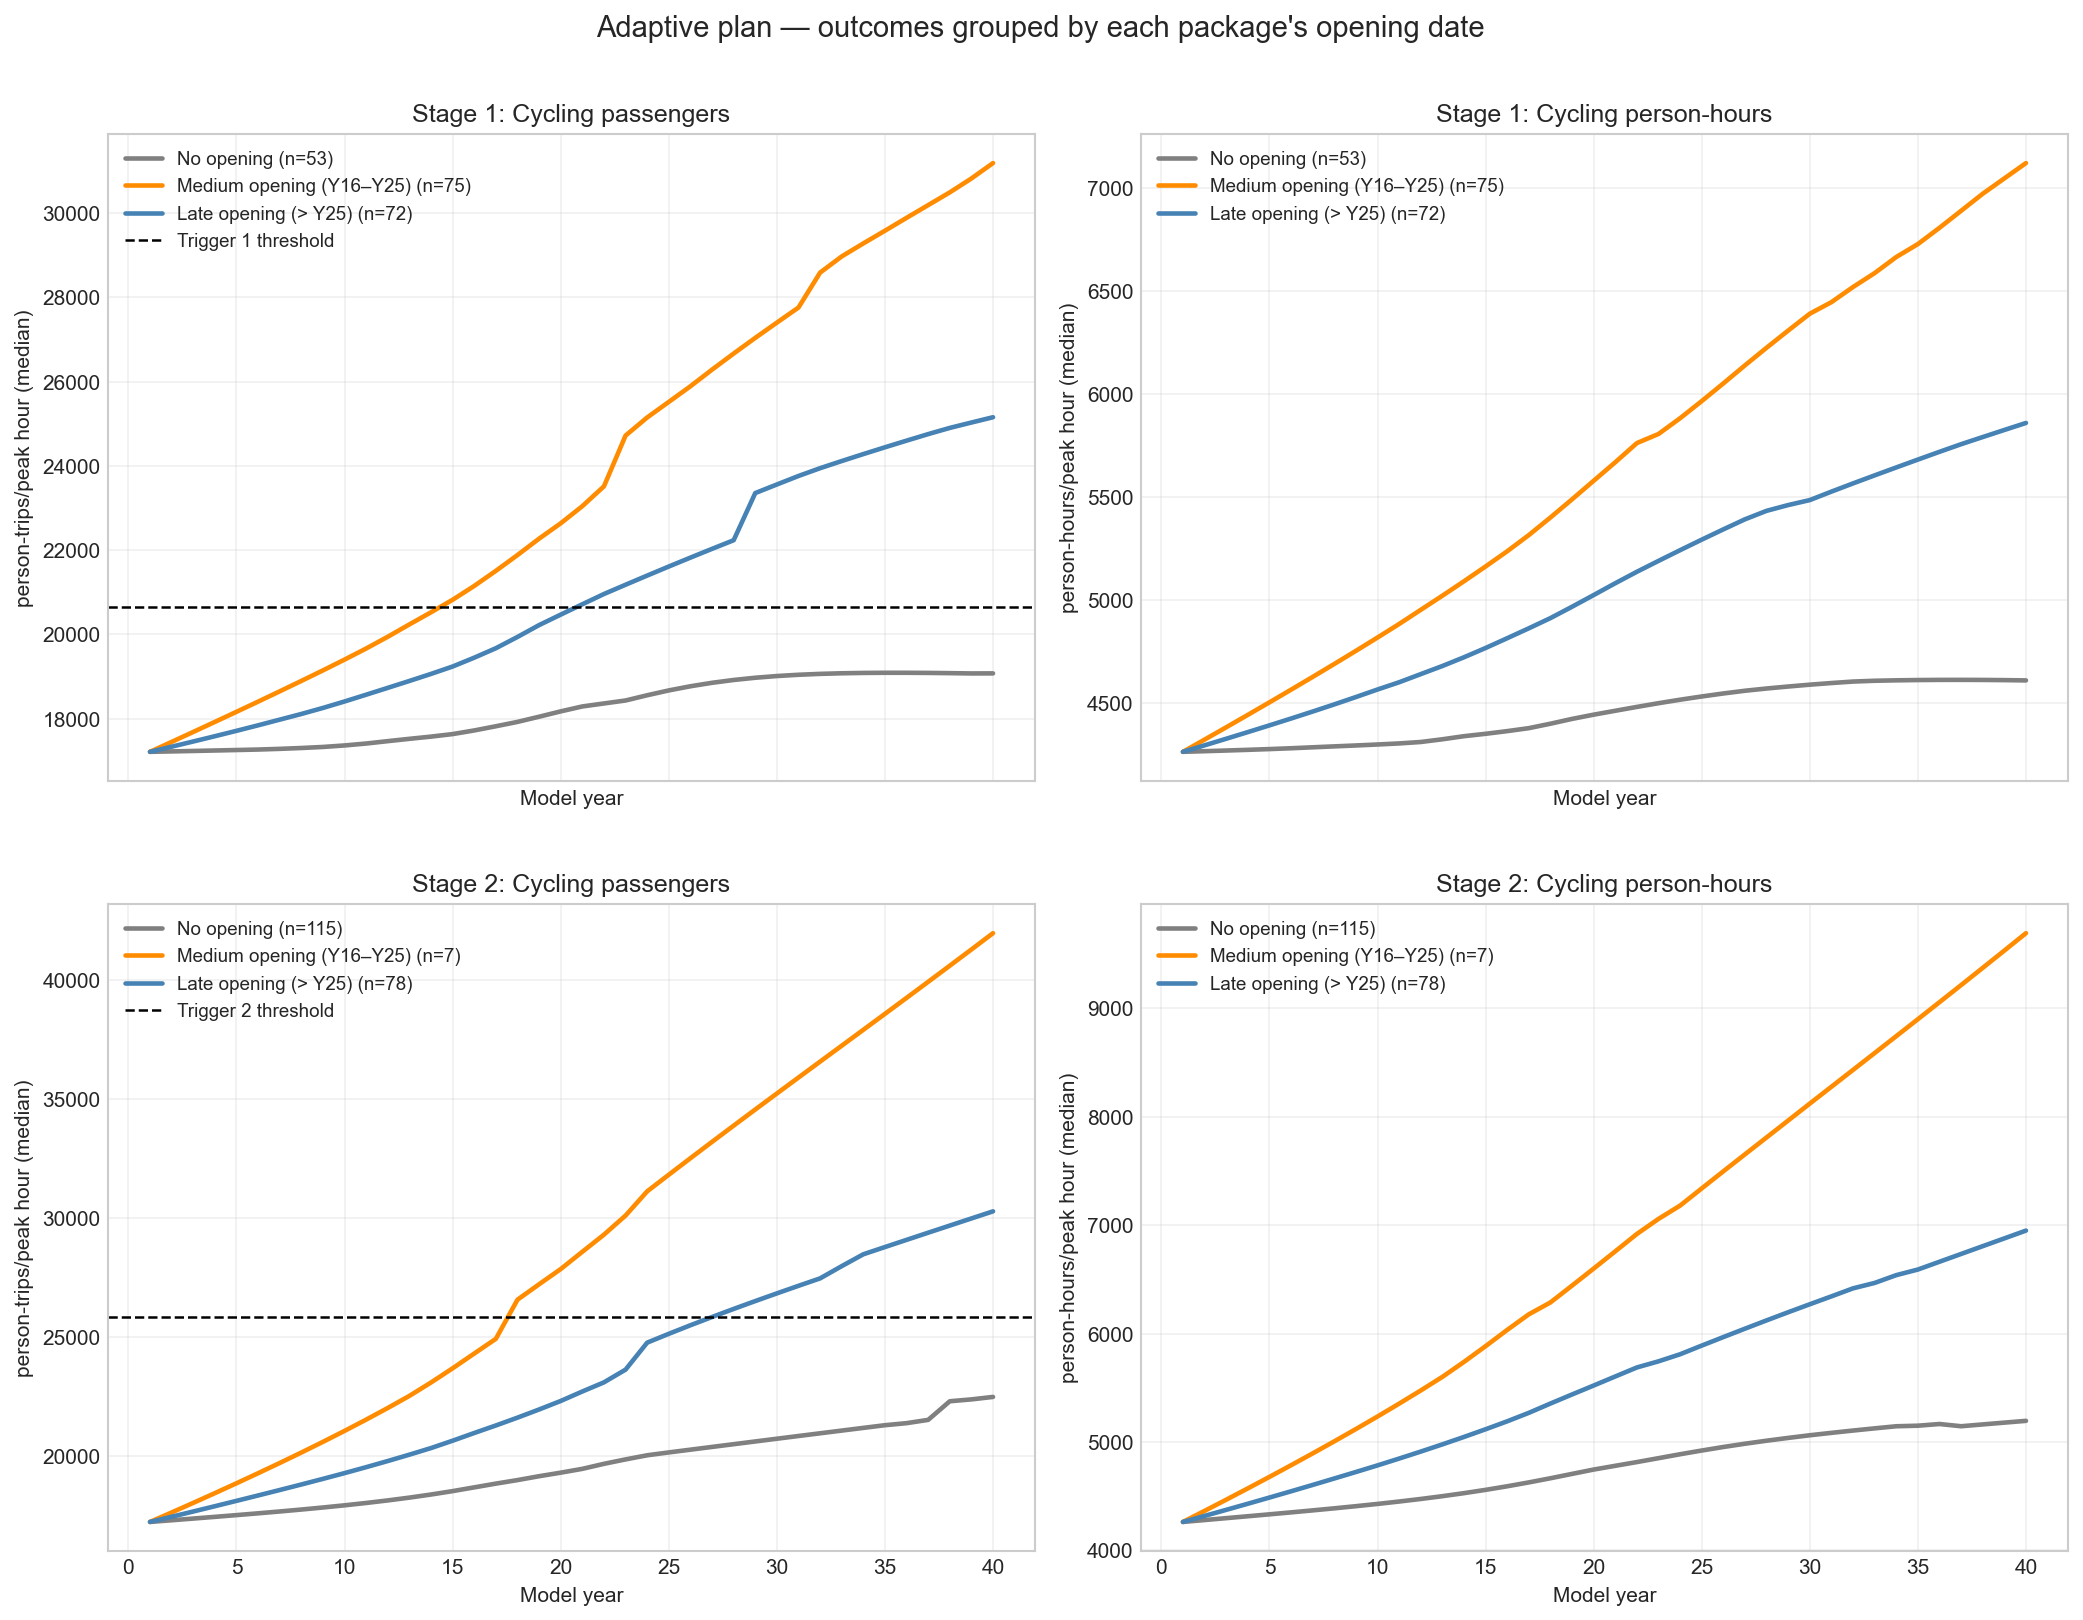
\includegraphics[width=\textwidth]{figures/scenario_triggers/04_adaptive_planning/04_adaptive_trigger_buckets.png}
\caption{NB04 with recalibrated triggers: monitored bike\_trips vs. the +20\%/+50\% threshold lines --- openings now distributed across scenarios.}
\end{figure}

\section{Takeaways}
\begin{enumerate}
\item \textbf{Build plans dominate on value; none is robust on the distance requirement.} Static2 is the value leader (+858\,MCHF NPV, 100\% positive, lowest regret 0) at $\approx$52\,MCHF capex; staged plans are close (+645/$+$648) at lower capex. All build plans meet all three requirements in only 3\% of scenarios; the distance requirement fails in $\approx$97.5\% everywhere.
\item \textbf{With the recalibrated triggers (+20\%/+50\% of the Year-1 baseline, persistence 3, lead 5/3) the adaptive plan now builds in a good share of growth scenarios}: Stage 1 activates in 73.5\% of scenarios, Stage 2 in 42.5\%, nothing in 26.5\%; its mean NPV rises from $-$2 to +164\,MCHF, while build plans stay at +574 to +858\,MCHF. Under the current requirements it still does not beat static/staged plans (joint success 3\%), because the failure wall is behavioural (BIKE\_ASC\_SHIFT), not timing.
\item \textbf{The binding uncertainty is behavioural, not demand.} BIKE\_ASC\_SHIFT (Sobol ST $\approx$0.96 on bike trip share) sets a clean failure threshold ($\approx$0.23 for the 20\% trip-share target); PASSENGER\_DEMAND\_GROWTH drives volumes, not shares. No infrastructure timing can move the preference wall.
\item \textbf{The retrained surrogate is healthy}: it now passes its strict OD gates (MAE 0.073\,/ RMSE 0.125\,min) after the corridor/stage/demand-domain changes, so NB04/NB05 results rest on a validated fast model.
\end{enumerate}

\end{document}
